\documentclass[hyperref={bookmarks=false},aspectratio=169]{beamer}
\usepackage{hyperref,ragged2e,amsmath,amssymb,url,bm}
\usepackage{graphicx,booktabs,array}
\usepackage{tikz}
\usetikzlibrary{shadows}
\usetikzlibrary{arrows.meta,positioning,calc,shapes.geometric,decorations.pathreplacing,matrix}
\graphicspath{{crops/}}
\usetheme{Goettingen}
% --- Paleta "Israel": celeste y azul del tejelet (Nm 15:38), oro del santuario, fondo crema ---
% (los nombres de color se conservan por compatibilidad con los cuerpos de las láminas: «ladrillo» = azul tejelet,
%  «cafe» = azul real, «cafeosc» = azul noche, «piedra» = celeste claro, «sepia» = azul pizarra)
\definecolor{cafe}{RGB}{26,82,150}
\definecolor{cafeosc}{RGB}{11,33,74}
\definecolor{tinta}{RGB}{20,32,56}
\definecolor{oro}{RGB}{206,162,52}
\definecolor{ladrillo}{RGB}{20,68,140}
\definecolor{piedra}{RGB}{234,243,251}
\definecolor{sepia}{RGB}{72,102,140}
\definecolor{celeste}{RGB}{96,166,222}
\setbeamercolor{structure}{fg=ladrillo}
\setbeamertemplate{sidebar canvas right}[vertical shading][top=celeste!75!ladrillo,middle=ladrillo,bottom=cafeosc]
\setbeamercolor{title in sidebar}{fg=oro!80!white}
\setbeamercolor{author in sidebar}{fg=piedra}
\setbeamercolor{section in sidebar}{fg=white}
\setbeamercolor{section in sidebar shaded}{fg=celeste!45!white}
\setbeamercolor{subsection in sidebar}{fg=white}
\setbeamercolor{subsection in sidebar shaded}{fg=celeste!45!white}
\let\raggedright\justifying
\definecolor{crema}{RGB}{250,245,230}
\setbeamertemplate{background canvas}[default]
\setbeamercolor{background canvas}{bg=crema}
\setbeamercolor{normal text}{fg=tinta}
\setbeamercolor{frametitle}{fg=ladrillo}
\setbeamerfont{frametitle}{series=\bfseries}
\setbeamertemplate{section in toc shaded}{\leavevmode{\color{sepia!85!black}\inserttocsection}\par}
\setbeamercolor{title}{fg=ladrillo}
\setbeamercolor{subtitle}{fg=cafe}
\setbeamercolor{item projected}{bg=cafe,fg=piedra}
\setbeamertemplate{itemize item}{\small\textcolor{oro!85!ladrillo}{$\blacktriangleright$}}
\setbeamertemplate{navigation symbols}{}
% --- Español + hebreo + griego (XeLaTeX) con fuentes empaquetadas en fonts/ ---
\usepackage[bidi=default]{babel}
\babelprovide[import,main]{spanish}
\babelprovide[import]{hebrew}
\babelprovide[import]{ancientgreek}
\babelfont[hebrew]{sf}[Path=fonts/, BoldFont=NotoHebrewSans-700.ttf]{NotoHebrewSans-400.ttf}
\babelfont[hebrew]{rm}[Path=fonts/, BoldFont=NotoHebrewSans-700.ttf]{NotoHebrewSans-400.ttf}
\babelfont[ancientgreek]{sf}[Path=fonts/]{GFSPorson.otf}
\babelfont[ancientgreek]{rm}[Path=fonts/]{GFSPorson.otf}
\newcommand{\heb}[1]{\mbox{\foreignlanguage{hebrew}{#1}}}
\newcommand{\grc}[1]{\foreignlanguage{ancientgreek}{#1}}
% --- Citas, imágenes, referencias ---
\usepackage[most]{tcolorbox}
\newtcolorbox{cita}[1][]{enhanced, colback=piedra!92!white, colframe=oro!90!ladrillo,
  boxrule=0pt, leftrule=2.5pt, arc=0pt, left=6pt, right=6pt, top=4pt, bottom=4pt,
  before skip=4pt, after skip=6pt, fontupper=\small\itshape, #1}
\newcommand{\fuente}[1]{\par\hfill{\upshape\bfseries\footnotesize\textcolor{ladrillo}{#1}}}
\newcommand{\imagen}[3][0.80]{%
  \centering\includegraphics[height=#1\textheight,width=\linewidth,keepaspectratio]{#2}\par\vspace{2pt}
  {\fontsize{5}{6}\selectfont\color{sepia}{\raggedleft\textit{Nota.} #3\par}}}
\makeatletter
\newcommand{\fotolado}[2]{%
  % Panel a la derecha, separado de la columna de texto (0.57): marco dorado, sombra y nota al pie.
  \begin{tikzpicture}[remember picture,overlay]
    \coordinate (fl) at ([xshift=\beamer@leftmargin+0.615\textwidth]current page.west);
    \coordinate (fr) at ([xshift=-\beamer@sidebarwidth-6pt]current page.east);
    \node[inner sep=0pt,anchor=center,draw=oro,line width=0.9pt,
      drop shadow={shadow xshift=1.2pt,shadow yshift=-1.2pt,opacity=0.30,fill=cafeosc}] (foto)
      at ([yshift=6pt]$(fl)!0.5!(fr)$)
      {\includegraphics[width=\dimexpr\paperwidth-\beamer@sidebarwidth-\beamer@leftmargin-0.615\textwidth-6pt\relax]{#1}};
    \node[anchor=north east,inner sep=0pt,text=sepia,font=\fontsize{4.6}{5.6}\selectfont,align=right,
      text width=\dimexpr\paperwidth-\beamer@sidebarwidth-\beamer@leftmargin-0.615\textwidth-6pt\relax]
      at ([yshift=-3pt]foto.south east) {\textit{Nota.} #2};
  \end{tikzpicture}}
\makeatother
\newcommand{\refapa}[1]{\par\hangindent=1.2em\hangafter=1\noindent #1\par\vspace{3pt}}
\usepackage{xurl}\urlstyle{same}
\newcommand{\destacar}[1]{\textbf{\textcolor{ladrillo}{#1}}}
% --- Piezas visuales de la serie: regla dorada bajo el título, notas y pies de figura ---
\addtobeamertemplate{frametitle}{}{\vspace{-3pt}{\color{oro}\rule{2.2cm}{1.1pt}}\vspace{1pt}}
\newtcolorbox{notalam}[1][Nota]{enhanced,colback=oro!10!white,colframe=oro!85!ladrillo,boxrule=0.5pt,arc=2pt,
  left=5pt,right=5pt,top=3pt,bottom=3pt,fonttitle=\bfseries\scriptsize,coltitle=cafeosc,colbacktitle=oro!30!white,
  fontupper=\scriptsize,title={#1},before skip=4pt,after skip=4pt}
\newtcolorbox{clave}[1][]{enhanced,colback=piedra,colframe=ladrillo,boxrule=0pt,leftrule=2.5pt,arc=0pt,
  left=5pt,right=5pt,top=3pt,bottom=3pt,fontupper=\scriptsize,before skip=4pt,after skip=4pt,#1}
\newcommand{\notafig}[1]{\par\vspace{2pt}{\fontsize{5}{6}\selectfont\color{sepia}\hfill\textit{Nota.} #1\par}}
\newcommand{\elabpropia}{\notafig{Elaboración propia.}}
\tikzset{hito/.style={circle,fill=oro,draw=white,line width=0.6pt,inner sep=1.6pt},
  etiq/.style={font=\tiny,text=tinta,align=center},
  flecha/.style={->,draw=oro!90!ladrillo,line width=1pt},
  bloque/.style={draw=ladrillo,line width=0.6pt,fill=piedra,rounded corners=3pt,font=\scriptsize,align=center,inner sep=4pt},
  bloqueoro/.style={draw=oro!90!ladrillo,line width=0.6pt,fill=oro!14!white,rounded corners=3pt,font=\scriptsize,align=center,inner sep=4pt},
  bloqueazul/.style={draw=cafeosc,fill=ladrillo,text=white,rounded corners=3pt,font=\scriptsize\bfseries,align=center,inner sep=4pt}}

\tikzset{caja/.style={draw=cafe!80!black,line width=0.7pt,top color=piedra!55!white,bottom color=piedra!92!oro,
  rounded corners=4pt,inner sep=5pt,font=\scriptsize,
  drop shadow={shadow xshift=0.7pt,shadow yshift=-0.8pt,opacity=0.25,fill=cafeosc}},
  >={Stealth[length=2.4mm,width=1.8mm]}, every picture/.style={line cap=round,line join=round}}
\newcommand{\precision}[1]{{\footnotesize\color{sepia}\textbf{Precisión:} #1}}
\newcommand{\pt}[2]{({#1-30},{#2-29})}
\title[Israel 6: Segundo Templo]{\bfseries{Israel, el pueblo de Dios}}
\subtitle{Estudio 6. El Israel del Segundo Templo}
\author{}\institute{}\date{}
\titlegraphic{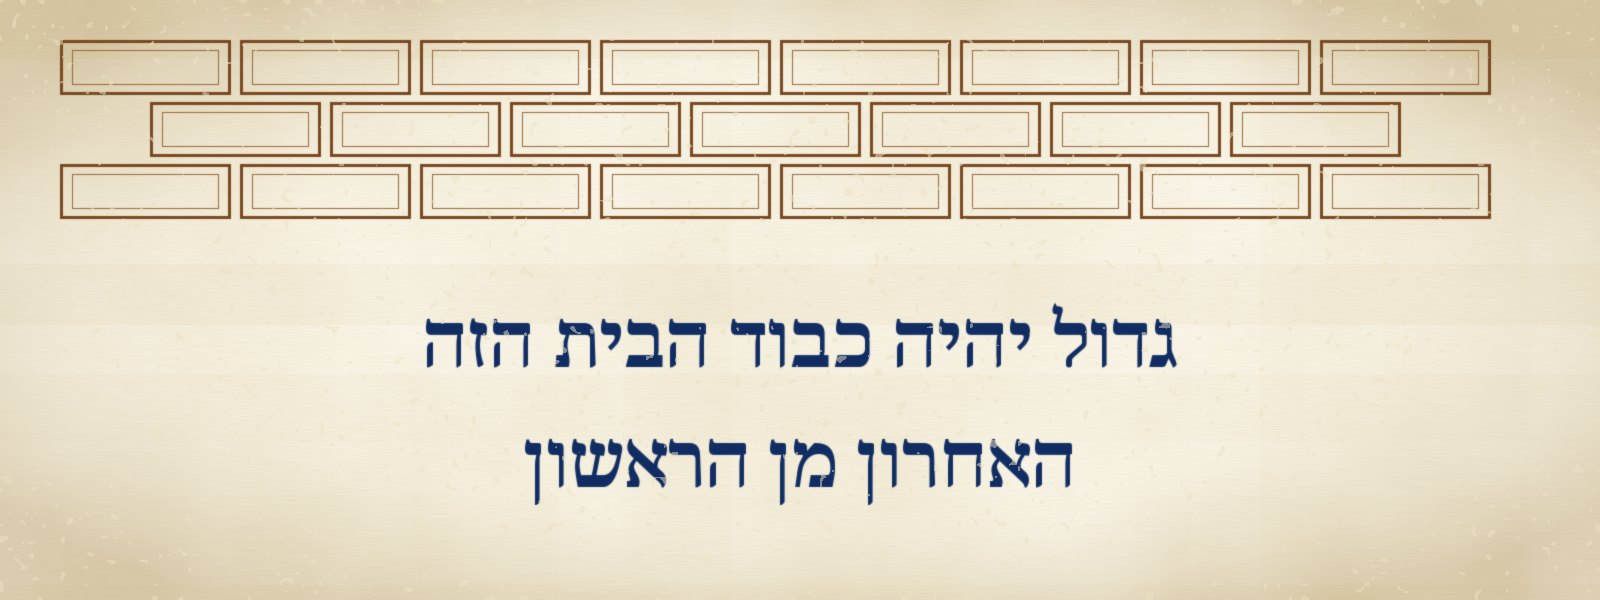
\includegraphics[width=0.85\linewidth,height=0.38\textheight,keepaspectratio]{portada.jpg}\\[-1pt]
  {\fontsize{5}{6}\selectfont\color{sepia}\textit{Nota.} Elaboración propia: Hag 2:9 en texto hebreo consonántico (BHS).}}
\begin{document}
\frame{\titlepage}

% ===================================================
\section{Introducción}
\begin{frame}{¿Volvió Israel del exilio?}
\begin{columns}[c,onlytextwidth]
\begin{column}{0.48\textwidth}
\begin{cita}He aquí que hoy somos siervos; en la tierra que diste a nuestros padres [\ldots] somos siervos en ella.\fuente{(Neh 9:36)}\end{cita}
\vspace{4pt}
\begin{cita}Señor, ¿restaurarás el reino a Israel en este tiempo?\fuente{(Hch 1:6)}\end{cita}
\end{column}
\begin{column}{0.48\textwidth}
\centering
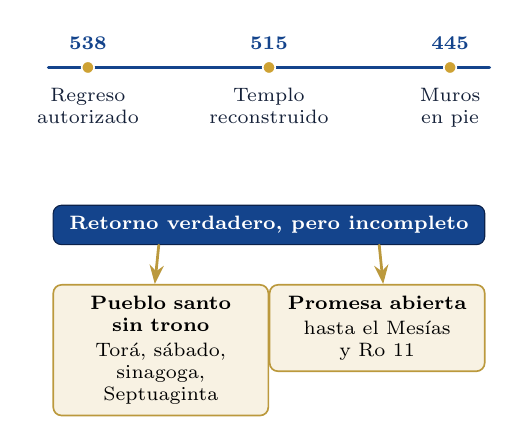
\begin{tikzpicture}[node distance=4mm]
\draw[line width=1.2pt,ladrillo] (0,0) -- (5.6,0);
\foreach \x/\a/\t in {0.5/538/{Regreso\\autorizado},2.8/515/{Templo\\reconstruido},5.1/445/{Muros\\en pie}}{
  \node[hito] at (\x,0) {};
  \node[etiq,above=3pt,font=\scriptsize\bfseries,text=ladrillo] at (\x,0) {\a};
  \node[etiq,below=4pt,font=\scriptsize] at (\x,0) {\t};}
\node[bloqueazul,text width=5.2cm] (r) at (2.8,-2.0) {Retorno verdadero, pero incompleto};
\node[bloqueoro,text width=2.45cm,anchor=north west] (a) at (0.05,-2.75) {\textbf{Pueblo santo sin trono}\\[1pt]Torá, sábado, sinagoga, Septuaginta};
\node[bloqueoro,text width=2.45cm,anchor=north east] (b) at (5.55,-2.75) {\textbf{Promesa abierta}\\[1pt]hasta el Mesías y Ro~11};
\draw[flecha] (r.south) ++(-1.4,0) -- (a.north -| 1.35,0);
\draw[flecha] (r.south) ++(1.4,0) -- (b.north -| 4.25,0);
\end{tikzpicture}
\elabpropia
\end{column}
\end{columns}
\end{frame}

\begin{frame}{Los ejes de la serie en esta etapa}
\centering
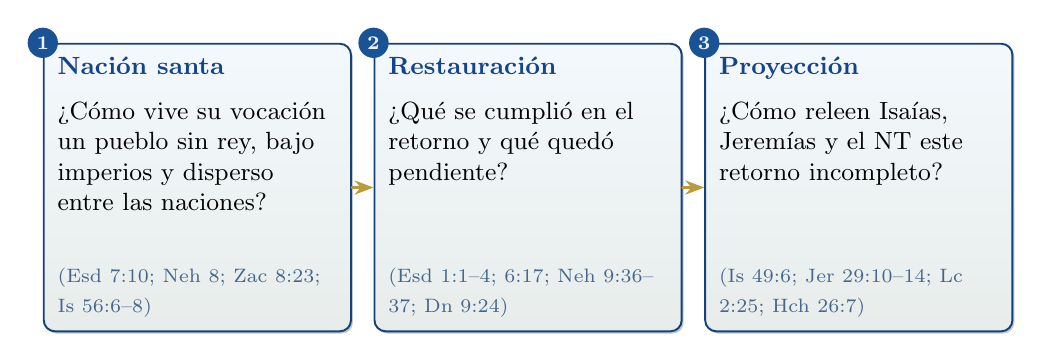
\begin{tikzpicture}
 \foreach \x/\n/\t/\d/\r in {0/1/{Nación santa}/{¿Cómo vive su vocación un pueblo sin rey, bajo imperios y disperso entre las naciones?}/{Esd 7:10; Neh 8; Zac 8:23; Is 56:6--8},
   4.2/2/{Restauración}/{¿Qué se cumplió en el retorno y qué quedó pendiente?}/{Esd 1:1--4; 6:17; Neh 9:36--37; Dn 9:24},
   8.4/3/{Proyección}/{¿Cómo releen Isaías, Jeremías y el NT este retorno incompleto?}/{Is 49:6; Jer 29:10--14; Lc 2:25; Hch 26:7}}{
  \node[caja,anchor=north] (b\n) at (\x,0) {\parbox[t][3.3cm][t]{3.55cm}{\RaggedRight
    {\small\textbf{\textcolor{ladrillo}{\t}}}\\[5pt]\small \d\par\vfill{\scriptsize\color{sepia}(\r)}}};
  \node[circle,fill=cafe,text=piedra,font=\scriptsize\bfseries,inner sep=1.6pt] at (b\n.north west) {\n};}
\draw[flecha] (b1.east) -- (b2.west);
\draw[flecha] (b2.east) -- (b3.west);
\end{tikzpicture}
\elabpropia
\vspace{8pt}
\begin{clave}Las citas bíblicas son traducción propia desde el texto hebreo y arameo (BHS) y griego (NA28). Numeración española [hebrea] cuando difiere.\end{clave}
\end{frame}

\begin{frame}{De doce tribus a «judíos»}
\centering
\begin{tikzpicture}[x=1cm,y=1cm]
\node[bloqueazul,text width=5.4cm] (isr) at (0,0) {Israel: las doce tribus, hijos de Jacob};
\node[bloque,text width=4.3cm] (n) at (-3.4,-1.25) {\textbf{Israel / reino del norte}\\diez tribus, Efraín, Samaria};
\node[bloque,text width=4.3cm] (s) at (3.4,-1.25) {\textbf{Judá / reino del sur}\\Judá y Benjamín, Jerusalén, casa de David};
\node[bloqueoro,text width=4.3cm] (n2) at (-3.4,-2.5) {Asiria, 722: dispersión};
\node[bloqueoro,text width=4.3cm] (s2) at (3.4,-2.5) {Babilonia, 586: exilio};
\node[bloque,text width=4.3cm,dashed] (n3) at (-3.4,-3.75) {No vuelve como cuerpo; norteños integrados en Judá (1~Cr 9:3)};
\node[bloque,text width=4.3cm] (s3) at (3.4,-3.75) {Retorno con Ciro (538): provincia persa \emph{Yehud} (Esd 1:5)};
\node[bloqueazul,text width=7.4cm] (j) at (0,-5.05) {«Judíos» (\heb{יְהוּדִים}) designa a todo el pueblo; ofrendas «por todo Israel» (Esd 6:17)};
\draw[flecha] (isr.south) -- ++(0,-0.3) -| (n.north);
\draw[flecha] (isr.south) -- ++(0,-0.3) -| (s.north);
\draw[flecha] (n) -- (n2); \draw[flecha] (s) -- (s2);
\draw[flecha] (n2) -- (n3); \draw[flecha] (s2) -- (s3);
\draw[flecha,dashed] (n3.east) -- (s3.west);
\draw[flecha] (s3.south) -- (s3.south |- j.north);
\end{tikzpicture}
\elabpropia
\end{frame}

\begin{frame}{Tres sentidos de «Israel»}
\centering\footnotesize\renewcommand{\arraystretch}{1.25}
\begin{tabular}{>{\RaggedRight\arraybackslash}p{2.4cm}>{\RaggedRight\arraybackslash}p{4.1cm}>{\RaggedRight\arraybackslash}p{5.0cm}}
\toprule
\color{ladrillo}\bfseries Término & \color{ladrillo}\bfseries Designa & \color{ladrillo}\bfseries En esta etapa\\\midrule
\textbf{Israel} (pueblo) & Las doce tribus, hijos de Jacob & La comunidad que vuelve se llama «todo Israel» (Esd 2:70; 6:17)\\
\textbf{Israel} (norte) & Diez tribus, Efraín, Samaria; deportado por Asiria (722) & No vuelve como cuerpo; norteños integrados en Judá (1~Cr 9:3); profecía de reunión (Zac 8:13; 10:6)\\
\textbf{Judá} (sur) & Judá y Benjamín, Jerusalén, casa de David; Babilonia (586) & Núcleo del retorno (Esd 1:5); provincia persa \emph{Yehud}\\
\textbf{Judíos} & \heb{יְהוּדִים}: «los de Judá» & Pasa a designar a todo el pueblo: Mardoqueo, benjaminita, es «judío» (Est 2:5)\\
\bottomrule
\end{tabular}
\elabpropia
\vspace{2pt}
\begin{clave}\textbf{Precisión:} en Esdras, Nehemías y Crónicas, «Israel» aplicado a los repatriados significa el pueblo completo.\end{clave}
\end{frame}

% ===================================================
\section{Cronología}
\begin{frame}{Del edicto de Ciro a Herodes}
\centering
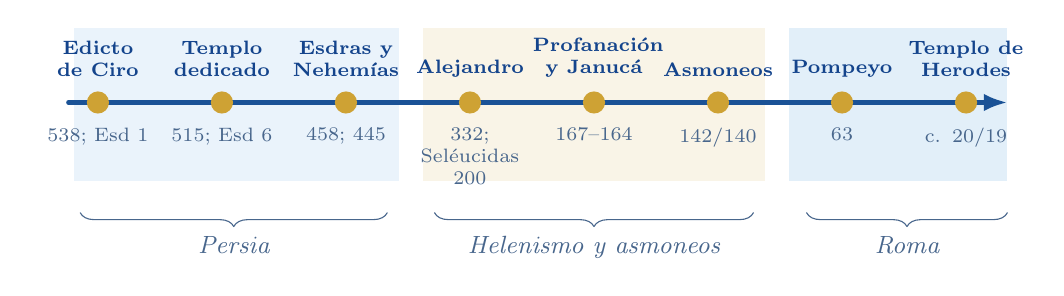
\begin{tikzpicture}[x=0.75cm]
\fill[piedra] (0.1,-1.0) rectangle (5.6,0.95);
\fill[oro!12!white] (6.0,-1.0) rectangle (11.8,0.95);
\fill[celeste!18!white] (12.2,-1.0) rectangle (15.9,0.95);
\draw[line width=1.6pt,cafe,-{Latex[length=3mm]}] (0,0) -- (15.9,0);
\foreach \x/\t/\b in {0.5/{Edicto de Ciro}/{538; Esd 1},
                      2.6/{Templo dedicado}/{515; Esd 6},
                      4.7/{Esdras y Nehemías}/{458; 445},
                      6.8/{Alejandro}/{332; Seléucidas 200},
                      8.9/{Profanación y Janucá}/{167--164},
                      11.0/{Asmoneos}/{142/140},
                      13.1/{Pompeyo}/{63},
                      15.2/{Templo de Herodes}/{c. 20/19}}{
  \fill[oro] (\x,0) circle (4pt);
  \node[above,font=\scriptsize\bfseries,text=ladrillo,text width=1.55cm,align=center] at (\x,0.2) {\t};
  \node[below,font=\scriptsize,text=sepia,text width=1.55cm,align=center] at (\x,-0.2) {\b};}
\draw[decorate,decoration={brace,amplitude=5pt,mirror},sepia] (0.2,-1.4) -- (5.4,-1.4) node[midway,below=5pt,font=\small\itshape]{Persia};
\draw[decorate,decoration={brace,amplitude=5pt,mirror},sepia] (6.2,-1.4) -- (11.6,-1.4) node[midway,below=5pt,font=\small\itshape]{Helenismo y asmoneos};
\draw[decorate,decoration={brace,amplitude=5pt,mirror},sepia] (12.5,-1.4) -- (15.9,-1.4) node[midway,below=5pt,font=\small\itshape]{Roma};
\end{tikzpicture}
\notafig{Elaboración propia. Fechas a.\,e.\,c.; varias están en debate.}
\vspace{10pt}
\begin{clave}El Segundo Templo se levanta en 515 a.\,e.\,c. y cae en 70 e.\,c.: cerca de seis siglos en que Israel vive bajo Persia, los reinos griegos, una dinastía propia y Roma.\end{clave}
\end{frame}

\begin{frame}{Fechas en debate}
\centering\footnotesize\renewcommand{\arraystretch}{1.25}
\begin{tabular}{>{\RaggedRight\arraybackslash}p{2.6cm}>{\RaggedRight\arraybackslash}p{4.6cm}>{\RaggedRight\arraybackslash}p{4.3cm}}
\toprule
\color{ladrillo}\bfseries Hecho & \color{ladrillo}\bfseries Dato bíblico o antiguo & \color{ladrillo}\bfseries Debate\\\midrule
Dedicación del templo & 3 de adar, año 6 de Darío~I (Esd 6:15) & Marzo de 515; algunos dan 516\\
Esdras & «Año séptimo de Artajerjes» (Esd 7:7) & Artajerjes~I: 458; Artajerjes~II: 398\\
Nehemías & Año 20 de Artajerjes (Neh 2:1) & 445/444\\
Profanación y Janucá & 15 kislev 145 y 25 kislev 148 de la era seléucida (1~Mac 1:54; 4:52) & Hoy 167--164; obras antiguas: 168--165\\
Templo de Herodes & Año 18 (\emph{Ant.} 15.380) / año 15 (\emph{Guerra} 1.401) & c. 20/19 o 23/22\\
Libro de Daniel & Siglo \textsc{vi} (tradición) & Redacción final c. 167--164 (crítica)\\
\bottomrule
\end{tabular}
\elabpropia
\end{frame}

% ===================================================
\section{Arqueología}
\begin{frame}{El mundo de la diáspora}
\begin{columns}[c,onlytextwidth]
\begin{column}{0.66\textwidth}\centering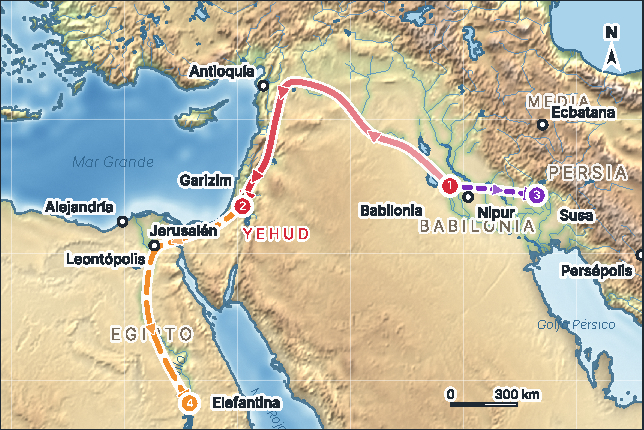
\includegraphics[width=\linewidth,height=0.86\textheight,keepaspectratio]{mapa_diaspora.pdf}\par\vspace{1pt}{\fontsize{4.5}{5.5}\selectfont\color{sepia}\textit{Nota.} Elaboración propia (GSHHS/WDB, Basemap); ubicaciones aproximadas.\par}\end{column}
\begin{column}{0.32\textwidth}\scriptsize\RaggedRight
{\scriptsize\RaggedRight
\definecolor{mapacarmesi}{HTML}{D62839}
\definecolor{mapanaranja}{HTML}{F28C28}
\definecolor{mapavioleta}{HTML}{7B2CBF}
\definecolor{mapaturquesa}{HTML}{0F8B8D}
\definecolor{mapaazul}{HTML}{1D4E89}
\definecolor{mapaocre}{HTML}{B5651D}
\tikz[baseline=-0.6ex]{\draw[white,line width=3.2pt,line cap=round](0,0)--(0.62,0);\draw[mapacarmesi,line width=1.8pt,line cap=round,-{Latex[length=1.6mm]}](0,0)--(0.62,0);}~El retorno: Babilonia $\to$ Jerusalén (Esd 1–2; 7–8)\par
\tikz[baseline=-0.6ex]{\draw[white,line width=3.2pt,line cap=round](0,0)--(0.62,0);\draw[mapavioleta,line width=1.8pt,line cap=round,dash pattern=on 1.4pt off 1.6pt,-{Latex[length=1.6mm]}](0,0)--(0.62,0);}~La corte persa: Susa (Est; Neh 1:1)\par
\tikz[baseline=-0.6ex]{\draw[white,line width=3.2pt,line cap=round](0,0)--(0.62,0);\draw[mapanaranja,line width=1.8pt,line cap=round,dash pattern=on 3.6pt off 2pt,-{Latex[length=1.6mm]}](0,0)--(0.62,0);}~Judíos en Egipto: hasta Elefantina (Jer 44:1)\par
\smallskip{\color{black!70}\textbf{Itinerario}}\par
\tikz[baseline=-0.7ex]\node[circle,fill=mapacarmesi,draw=white,line width=0.5pt,text=white,font=\fontsize{5}{5}\selectfont\bfseries,inner sep=0.6pt,minimum size=2.6mm]{1};\,Babilonia\quad \tikz[baseline=-0.7ex]\node[circle,fill=mapacarmesi,draw=white,line width=0.5pt,text=white,font=\fontsize{5}{5}\selectfont\bfseries,inner sep=0.6pt,minimum size=2.6mm]{2};\,Jerusalén\quad \tikz[baseline=-0.7ex]\node[circle,fill=mapavioleta,draw=white,line width=0.5pt,text=white,font=\fontsize{5}{5}\selectfont\bfseries,inner sep=0.6pt,minimum size=2.6mm]{3};\,Susa\quad \tikz[baseline=-0.7ex]\node[circle,fill=mapanaranja,draw=white,line width=0.5pt,text=white,font=\fontsize{5}{5}\selectfont\bfseries,inner sep=0.6pt,minimum size=2.6mm]{4};\,Elefantina\par}

\end{column}
\end{columns}
\end{frame}

\begin{frame}{El mundo de la diáspora: claves}
\begin{columns}[c,onlytextwidth]
\begin{column}{0.42\textwidth}\footnotesize\RaggedRight
\textbf{\textcolor{ladrillo}{El retorno}} sigue el Éufrates y baja por Siria: unos 1.400 km (Esd 1--2; 7--8).\par\medskip
\textbf{\textcolor{ladrillo}{Babilonia}}: Al-Yahudu (sitio exacto desconocido); archivo de Murashu en Nipur.\par\medskip
\textbf{\textcolor{ladrillo}{Susa}}: Ester; Nehemías, copero del rey.\par\medskip
\textbf{\textcolor{ladrillo}{Ecbatana}}: memorándum de Ciro (Esd 6:2).\par\medskip
\textbf{\textcolor{ladrillo}{Egipto}}: Elefantina, Leontópolis, Alejandría.
\end{column}
\begin{column}{0.54\textwidth}\centering
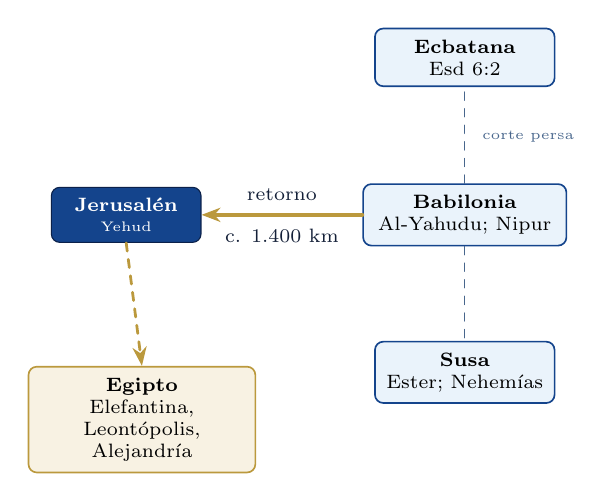
\begin{tikzpicture}[x=1cm,y=1cm]
\node[bloqueazul,minimum width=1.9cm] (jer) at (0,0) {Jerusalén\\[-1pt]{\tiny\mdseries Yehud}};
\node[bloque,text width=2.3cm] (bab) at (4.3,0) {\textbf{Babilonia}\\Al-Yahudu; Nipur};
\node[bloque,text width=2.0cm] (ecb) at (4.3,2.0) {\textbf{Ecbatana}\\Esd 6:2};
\node[bloque,text width=2.0cm] (sus) at (4.3,-2.0) {\textbf{Susa}\\Ester; Nehemías};
\node[bloqueoro,text width=2.6cm] (egi) at (0.2,-2.6) {\textbf{Egipto}\\Elefantina, Leontópolis, Alejandría};
\draw[flecha,line width=1.4pt] (bab.west) -- node[etiq,above=1pt,font=\scriptsize]{retorno} node[etiq,below=1pt,font=\scriptsize]{c. 1.400 km} (jer.east);
\draw[sepia,dashed] (bab) -- (ecb); \draw[sepia,dashed] (bab) -- (sus);
\draw[flecha,dashed] (jer.south) -- (egi.north);
\node[etiq,font=\tiny,text=sepia,anchor=west] at (4.4,1.0) {corte persa};
\end{tikzpicture}
\elabpropia
\end{column}
\end{columns}
\end{frame}

\begin{frame}{Babilonia y Egipto}
\centering
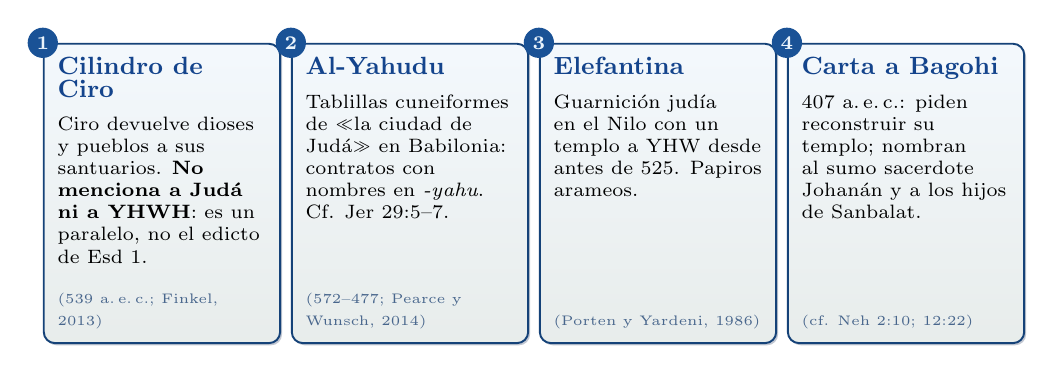
\begin{tikzpicture}
 \foreach \x/\n/\t/\d/\r in {0/1/{Cilindro de Ciro}/{Ciro devuelve dioses y pueblos a sus santuarios. \textbf{No menciona a Judá ni a YHWH}: es un paralelo, no el edicto de Esd 1.}/{539 a.\,e.\,c.; Finkel, 2013},
   3.15/2/{Al-Yahudu}/{Tablillas cuneiformes de «la ciudad de Judá» en Babilonia: contratos con nombres en \emph{-yahu}. Cf. Jer 29:5--7.}/{572--477; Pearce y Wunsch, 2014},
   6.3/3/{Elefantina}/{Guarnición judía en el Nilo con un templo a YHW desde antes de 525. Papiros arameos.}/{Porten y Yardeni, 1986},
   9.45/4/{Carta a Bagohi}/{407 a.\,e.\,c.: piden reconstruir su templo; nombran al sumo sacerdote Johanán y a los hijos de Sanbalat.}/{cf. Neh 2:10; 12:22}}{
  \node[caja,anchor=north] (b\n) at (\x,0) {\parbox[t][3.45cm][t]{2.65cm}{\RaggedRight
    {\small\textbf{\textcolor{ladrillo}{\t}}}\\[4pt]\scriptsize \d\par\vfill{\tiny\color{sepia}(\r)}}};
  \node[circle,fill=cafe,text=piedra,font=\scriptsize\bfseries,inner sep=1.6pt] at (b\n.north west) {\n};}
\end{tikzpicture}
\elabpropia
\begin{notalam}[Una diáspora fiel, con matices]
La mayoría de los desterrados había echado raíces, como pidió Jer 29:5--7, y no volvió. En Elefantina hay fidelidad al Dios de Israel, pero con un templo fuera de Jerusalén y menciones de otras divinidades junto a YHW. La carta a Bagohi confirma, además, la existencia de Sanbalat, adversario de Nehemías.
\end{notalam}
\end{frame}

\begin{frame}{Yehud y Samaria en el período persa}
\begin{columns}[T,onlytextwidth]
\begin{column}{0.48\textwidth}\footnotesize
\begin{itemize}
\item \textbf{Sellos y monedas \emph{yhd}}: la provincia de Yehud; una moneda de «Ezequías el gobernador» (Lipschits y Vanderhooft, 2011; Meshorer, 2001).\medskip
\item \textbf{Una Jerusalén poco poblada}: «la ciudad era espaciosa y grande, pero poco pueblo dentro de ella» (Neh 7:4); repoblada por sorteo (Neh 11:1).\medskip
\item \textbf{Garizim}: recinto samaritano del s. \textsc{v} a.\,e.\,c., destruido por Juan Hircano c. 112/111 (Magen, 2008; cf. Jn 4:20).
\end{itemize}
\end{column}
\begin{column}{0.48\textwidth}
\begin{notalam}[Debate abierto: el muro de Nehemías]
\footnotesize
E. Mazar (2005--2007) le atribuyó una torre y un tramo de muro en la ladera oriental de la Ciudad de David.\par\smallskip
Finkelstein (2008) los fecha en época asmonea y piensa que Neh 3 refleja en parte una realidad posterior.\par\smallskip
Otros responden que Nehemías reparó sobre todo trazados antiguos.
\end{notalam}
\begin{notalam}[Garizim, antes de lo que se creía]
\footnotesize Josefo situaba su fundación en tiempos de Alejandro (\emph{Ant.} 11.302--347); la arqueología la adelanta más de un siglo.
\end{notalam}
\end{column}
\end{columns}
\end{frame}

\begin{frame}{Hallazgos helenísticos y romanos}
\centering
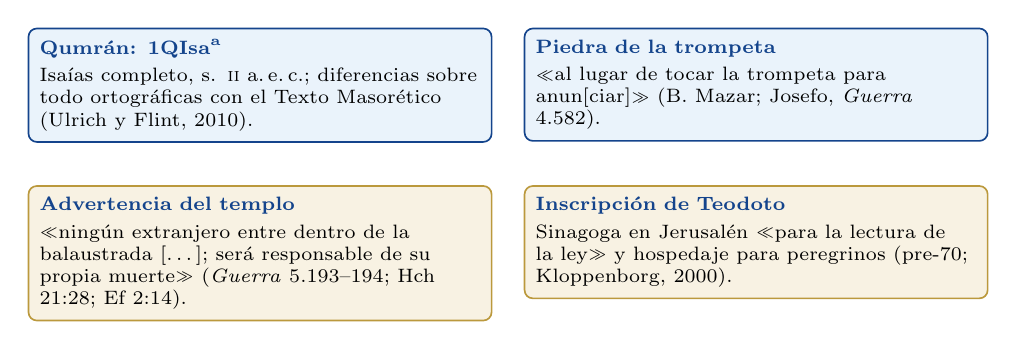
\begin{tikzpicture}[x=1cm,y=1cm]
\node[bloque,text width=5.6cm,align=left,anchor=north west] (q) at (0,0) {\textbf{\textcolor{ladrillo}{Qumrán: 1QIsa\textsuperscript{a}}}\\[2pt]Isaías completo, s. \textsc{ii} a.\,e.\,c.; diferencias sobre todo ortográficas con el Texto Masorético (Ulrich y Flint, 2010).};
\node[bloque,text width=5.6cm,align=left,anchor=north west] (t) at (6.3,0) {\textbf{\textcolor{ladrillo}{Piedra de la trompeta}}\\[2pt]«al lugar de tocar la trompeta para anun[ciar]» (B. Mazar; Josefo, \emph{Guerra} 4.582).};
\node[bloqueoro,text width=5.6cm,align=left,anchor=north west] (a) at (0,-2.0) {\textbf{\textcolor{ladrillo}{Advertencia del templo}}\\[2pt]«ningún extranjero entre dentro de la balaustrada [\ldots]; será responsable de su propia muerte» (\emph{Guerra} 5.193--194; Hch 21:28; Ef 2:14).};
\node[bloqueoro,text width=5.6cm,align=left,anchor=north west] (d) at (6.3,-2.0) {\textbf{\textcolor{ladrillo}{Inscripción de Teodoto}}\\[2pt]Sinagoga en Jerusalén «para la lectura de la ley» y hospedaje para peregrinos (pre-70; Kloppenborg, 2000).};
\end{tikzpicture}
\elabpropia
\vspace{6pt}
\begin{clave}Las promesas de Isaías que este estudio sigue se leían entonces casi como hoy; la balaustrada será el trasfondo del «muro intermedio de separación» (Ef 2:14).\end{clave}
\end{frame}

% ===================================================
\section{Período persa}
\begin{frame}{Ciro, «su ungido»}
\fotolado{panel_is44.jpg}{Elaboración propia: Is 44:28 y 45:1 en texto hebreo consonántico (BHS).}
\begin{columns}[c,onlytextwidth]
\begin{column}{0.57\textwidth}
\begin{cita}En el primer año de Ciro, para que se cumpliera la palabra de YHWH por boca de Jeremías, YHWH despertó el espíritu de Ciro [\ldots]: «Quien haya entre vosotros de todo su pueblo, sea su Dios con él, y suba».\fuente{(Esd 1:1--3; 2 Cr 36:22--23)}\end{cita}
\scriptsize
\begin{itemize}
\item Is 45:1: \heb{לִמְשִׁיחוֹ לְכוֹרֶשׁ}, «a su ungido, a Ciro»: único rey extranjero llamado \emph{mashíaj}.
\item Sesbasar, «príncipe de Judá» (Esd 1:8); luego Zorobabel, nieto de Joaquín, y el sumo sacerdote Josué.
\item Ancianos que lloran ante los cimientos (Esd 3:12); obra detenida hasta 520 (Esd 4).
\end{itemize}
\end{column}
\begin{column}{0.41\textwidth}\end{column}
\end{columns}
\end{frame}

\begin{frame}{¿Quiénes vuelven?}
\begin{columns}[T,onlytextwidth]
\begin{column}{0.48\textwidth}
\centering{\heb{וצפירי עזין לחטאה על כל ישראל}}\par\smallskip
\begin{cita}Y como ofrenda por el pecado por todo Israel, doce machos cabríos, conforme al número de las tribus de Israel.\fuente{(Esd 6:17)}\end{cita}
\begin{notalam}[Precisión]
No vuelven las diez tribus como tales, sino norteños integrados en Judá (2~Cr 15:9; 30:11; 34:9). El paralelo de Neh 11:3--19 solo nombra a Judá y Benjamín, y hay quien lee 1~Cr 9:3 como reflejo de la visión del Cronista.
\end{notalam}
\end{column}
\begin{column}{0.48\textwidth}\centering
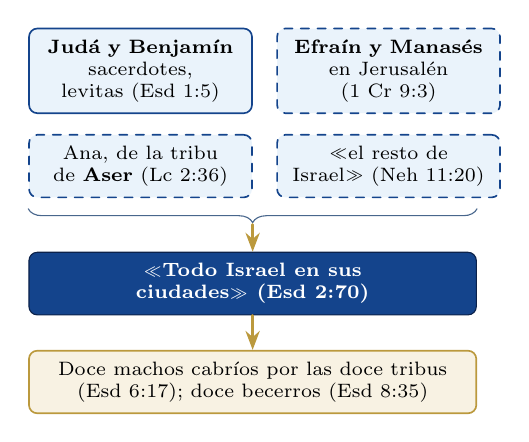
\begin{tikzpicture}[x=1cm,y=1cm]
\node[bloque,text width=2.55cm,anchor=north west] (a) at (0,0) {\textbf{Judá y Benjamín}\\sacerdotes, levitas (Esd 1:5)};
\node[bloque,text width=2.55cm,anchor=north west,dashed] (b) at (3.15,0) {\textbf{Efraín y Manasés}\\en Jerusalén (1~Cr 9:3)};
\node[bloque,text width=2.55cm,anchor=north west,dashed] (c) at (3.15,-1.35) {«el resto de Israel» (Neh 11:20)};
\node[bloque,text width=2.55cm,anchor=north west,dashed] (d) at (0,-1.35) {Ana, de la tribu de \textbf{Aser} (Lc 2:36)};
\node[bloqueazul,text width=5.4cm] (t) at (2.85,-3.25) {«Todo Israel en sus ciudades» (Esd 2:70)};
\node[bloqueoro,text width=5.4cm] (o) at (2.85,-4.5) {Doce machos cabríos por las doce tribus (Esd 6:17); doce becerros (Esd 8:35)};
\draw[decorate,decoration={brace,amplitude=5pt,mirror},sepia] (0,-2.3) -- (5.7,-2.3);
\draw[flecha] (2.85,-2.5) -- (t.north);
\draw[flecha] (t) -- (o);
\end{tikzpicture}
\notafig{Elaboración propia. Línea discontinua: presencia norteña minoritaria.}
\end{column}
\end{columns}
\end{frame}

\begin{frame}{El nombre «judío»}
\centering{\large\heb{אִישׁ יְהוּדִי} [\ldots] \heb{אִישׁ יְמִינִי}}\par
{\footnotesize «un judío [\ldots] benjaminita» (Est 2:5)}\par\vspace{8pt}
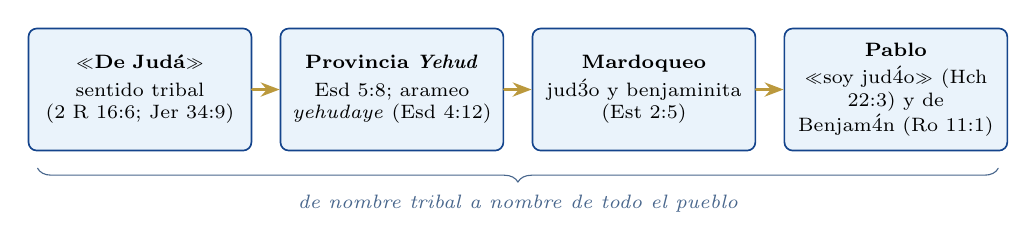
\begin{tikzpicture}[x=1cm,y=1cm]
\foreach \i/\x/\t/\d in {1/0/{«De Judá»}/{sentido tribal\\(2~R 16:6; Jer 34:9)},
  2/3.2/{Provincia \emph{Yehud}}/{Esd 5:8; arameo \emph{yehudaye} (Esd 4:12)},
  3/6.4/{Mardoqueo}/{judío y benjaminita\\(Est 2:5)},
  4/9.6/{Pablo}/{«soy judío» (Hch 22:3) y de Benjamín (Ro 11:1)}}{
  \node[bloque,text width=2.55cm,minimum height=1.55cm] (n\i) at (\x,0) {\textbf{\t}\\[2pt]\d};}
\foreach \a/\b in {1/2,2/3,3/4}{\draw[flecha] (n\a.east) -- (n\b.west);}
\draw[decorate,decoration={brace,amplitude=5pt,mirror},sepia] (-1.3,-1.0) -- (10.9,-1.0)
  node[midway,below=6pt,font=\scriptsize\itshape,text=sepia]{de nombre tribal a nombre de todo el pueblo};
\end{tikzpicture}
\elabpropia
\vspace{6pt}
\begin{clave}Josefo: se llaman «judíos» desde que subieron de Babilonia, por la tribu de Judá (\emph{Ant.} 11.173). En el NT, \grc{Ἰουδαῖος} designa a todo el pueblo.\end{clave}
\end{frame}

\begin{frame}{Los samaritanos}
\centering
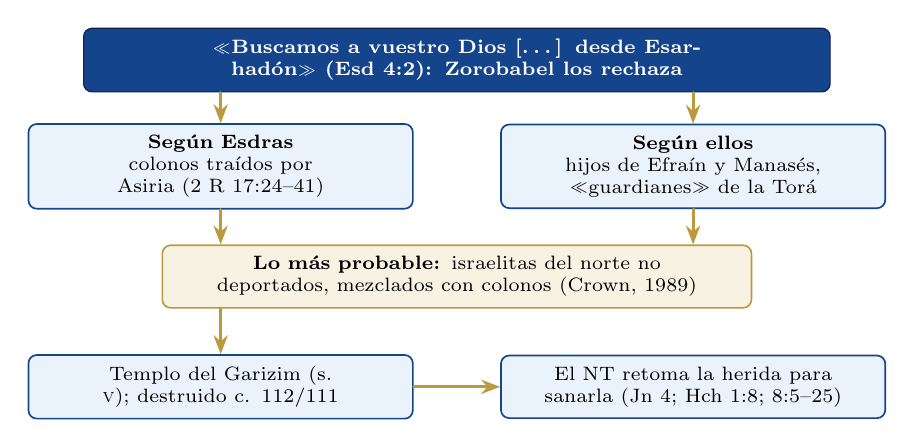
\begin{tikzpicture}[x=1cm,y=1cm]
\node[bloqueazul,text width=9.2cm] (p) at (0,0) {«Buscamos a vuestro Dios [\ldots] desde Esar-hadón» (Esd 4:2): Zorobabel los rechaza};
\node[bloque,text width=4.6cm] (e) at (-3.0,-1.35) {\textbf{Según Esdras}\\colonos traídos por Asiria (2~R 17:24--41)};
\node[bloque,text width=4.6cm] (s) at (3.0,-1.35) {\textbf{Según ellos}\\hijos de Efraín y Manasés, «guardianes» de la Torá};
\node[bloqueoro,text width=7.2cm] (m) at (0,-2.75) {\textbf{Lo más probable:} israelitas del norte no deportados, mezclados con colonos (Crown, 1989)};
\node[bloque,text width=4.6cm] (g) at (-3.0,-4.15) {Templo del Garizim (s. \textsc{v}); destruido c. 112/111};
\node[bloque,text width=4.6cm] (n) at (3.0,-4.15) {El NT retoma la herida para sanarla (Jn 4; Hch 1:8; 8:5--25)};
\draw[flecha] (p.south) ++(-3,0) -- (e.north);
\draw[flecha] (p.south) ++(3,0) -- (s.north);
\draw[flecha] (e.south) -- (e.south |- m.north);
\draw[flecha] (s.south) -- (s.south |- m.north);
\draw[flecha] (m.south -| g.north) -- (g.north);
\draw[flecha] (g) -- (n);
\end{tikzpicture}
\elabpropia
\end{frame}

\begin{frame}{Hageo: la gloria postrera}
\centering{\large\heb{גָּדוֹל יִהְיֶה כְּבוֹד הַבַּיִת הַזֶּה הָאַחֲרוֹן מִן־הָרִאשׁוֹן}}\par\smallskip
\begin{cita}Haré temblar a todas las naciones, y vendrá lo precioso de todas las naciones, y llenaré de gloria esta casa [\ldots]. Mayor será la gloria de esta casa postrera que la de la primera [\ldots], y en este lugar daré paz.\fuente{(Hag 2:7--9)}\end{cita}
\begin{columns}[T,onlytextwidth]
\begin{column}{0.48\textwidth}
\begin{notalam}[Hebreo: \heb{חֶמְדַּת כָּל־הַגּוֹיִם}]
«Lo deseable de todas las naciones», con verbo en plural; es decir, sus tesoros (cf. Is 60:5). La Vulgata tradujo \emph{desideratus}, «el deseado», base de la lectura mesiánica tradicional.
\end{notalam}
\end{column}
\begin{column}{0.48\textwidth}
\begin{clave}\textbf{Zorobabel, «anillo de sellar»} (Hag 2:23): inversión de Jer 22:24. La casa de David sigue elegida, aunque Zorobabel no llega a reinar.\end{clave}
\end{column}
\end{columns}
\end{frame}

\begin{frame}{Zacarías: dos casas}
\fotolado{panel_zac8.jpg}{Elaboración propia: Zac 8:23 en texto hebreo consonántico (BHS).}
\begin{columns}[c,onlytextwidth]
\begin{column}{0.57\textwidth}
\begin{cita}Como fuisteis maldición entre las naciones, oh \textbf{casa de Judá y casa de Israel}, así os salvaré y seréis bendición.\fuente{(Zac 8:13)}\end{cita}
\scriptsize
\begin{itemize}
\item \textbf{Zac 2:11--12 [2:15--16]}: muchas naciones se unen a YHWH; Judá, su porción en la \heb{אַדְמַת הַקֹּדֶשׁ}, «tierra santa».
\item \textbf{Zac 9:13; 10:6}: Judá y Efraín, Judá y José.
\item \textbf{Zac 9:9}: el rey viene \heb{עָנִי}, «humilde», sobre un asno.
\item \textbf{Zac 12:10}: «mirarán a mí, a quien traspasaron» (Jn 19:37).
\end{itemize}
\end{column}
\begin{column}{0.41\textwidth}\end{column}
\end{columns}
\end{frame}

\begin{frame}{Ester y Purim}
\begin{columns}[T,onlytextwidth]
\begin{column}{0.48\textwidth}
\begin{cita}Hay un pueblo esparcido y dividido entre los pueblos en todas las provincias de tu reino, y sus leyes son diferentes.\fuente{(Est 3:8)}\end{cita}
\small Susa, bajo Asuero (Jerjes~I, 486--465). Purim: 14 y 15 de adar (Est 9:20--32).\par\medskip
\begin{clave}\textbf{Precisión:} algunos detalles históricos se discuten, pero la corte persa está retratada con exactitud.\end{clave}
\end{column}
\begin{column}{0.48\textwidth}\footnotesize
\begin{itemize}
\item El hebreo de Ester \textbf{no menciona a Dios}. Talmud: «yo esconderé (\emph{haster astir}) mi rostro» (Dt 31:18; Julín 139b).\medskip
\item «Muchos de los pueblos de la tierra \heb{מִתְיַהֲדִים}», \emph{se hacían judíos} (Est 8:17); LXX: «se circuncidaban y judaizaban».\medskip
\item 2~Mac 15:36: «el día de Mardoqueo», primera mención de Purim fuera de Ester.
\end{itemize}
\end{column}
\end{columns}
\end{frame}

\begin{frame}{Esdras y Nehemías: un pueblo en torno a un libro}
\centering{\heb{וַיִּקְרְאוּ בַסֵּפֶר בְּתוֹרַת הָאֱלֹהִים מְפֹרָשׁ וְשׂוֹם שֶׂכֶל}}\par\smallskip
\begin{cita}Y leían en el libro de la ley de Dios con claridad, y ponían el sentido, de modo que entendían la lectura.\fuente{(Neh 8:8)}\end{cita}
\vspace{8pt}
\begin{columns}[T,onlytextwidth]
\begin{column}{0.48\textwidth}\footnotesize
\textbf{\textcolor{ladrillo}{Esdras}}, escriba: «preparó su corazón para \emph{inquirir} la ley, cumplirla y enseñar» (Esd 7:10). Llega c. 458 (o 398).
\end{column}
\begin{column}{0.48\textwidth}\footnotesize
\textbf{\textcolor{ladrillo}{Nehemías}}, copero de Artajerjes~I: muros en 52 días (Neh 6:15) frente a Sanbalat, Tobías y Gesem.\par\smallskip
Reformas: sábado (Neh 13:15--22) y matrimonios mixtos; el motivo es la idolatría (Neh 13:26), no la etnia.
\end{column}
\end{columns}
\end{frame}

\begin{frame}{De la lectura al pacto (Neh 8--10)}
\centering
\begin{tikzpicture}[x=1cm,y=1cm]
\foreach \i/\t/\d in {1/{Lectura}/{pública y explicada (Neh 8:1--8)},
  2/{Llanto y gozo}/{«el gozo de YHWH es vuestra fuerza» (8:10)},
  3/{Sucot}/{como no se hacía desde Josué (8:17)},
  4/{Confesión}/{pecados de los padres (Neh 9)},
  5/{Pacto escrito}/{\heb{אֲמָנָה} (9:38 [10:1])}}{
  \node[bloque,text width=2.0cm,minimum height=1.75cm] (n\i) at ({(\i-1)*2.55},0) {\textbf{\textcolor{ladrillo}{\t}}\\[2pt]\d};
  \node[circle,fill=cafe,text=piedra,font=\scriptsize\bfseries,inner sep=1.4pt] at (n\i.north west) {\i};}
\foreach \a/\b in {1/2,2/3,3/4,4/5}{\draw[flecha] (n\a.east) -- (n\b.west);}
\end{tikzpicture}
\elabpropia
\vspace{8pt}
\begin{notalam}[Hebreo: \heb{לִדְרוֹשׁ}, «inquirir» (Esd 7:10)]
\footnotesize Es el verbo del que vendrá \emph{midrash}. El orden del versículo pone primero el estudio, luego el cumplimiento y solo entonces la enseñanza. Un pueblo se reconstituye en torno a un libro.
\end{notalam}
\end{frame}

\begin{frame}{Malaquías y Elías}
\fotolado{panel_mal3.jpg}{Elaboración propia: Mal 3:1 en texto hebreo consonántico (BHS).}
\begin{columns}[c,onlytextwidth]
\begin{column}{0.57\textwidth}
\begin{cita}He aquí que yo envío mi mensajero, y preparará el camino delante de mí; y vendrá súbitamente a su templo el Señor a quien vosotros buscáis.\fuente{(Mal 3:1)}\end{cita}
\scriptsize
\begin{itemize}
\item \textbf{Mal 1:11}: «grande es mi nombre entre las naciones».
\item \textbf{Mal 3:6}: «yo, YHWH, no cambio; por eso vosotros, hijos de Jacob, no habéis sido consumidos».
\item \textbf{Mal 4:4--6 [3:22--24]}: «acordaos de la ley de Moisés»; Elías hará volver el corazón de los padres a los hijos (Lc 1:17).
\end{itemize}
\end{column}
\begin{column}{0.41\textwidth}\end{column}
\end{columns}
\end{frame}

% ===================================================
\section{Los 400 años}
\begin{frame}{¿Cuatrocientos años de silencio?}
\begin{columns}[T,onlytextwidth]
\begin{column}{0.44\textwidth}\footnotesize
\textbf{\textcolor{ladrillo}{Sin profeta canónico}}
\begin{itemize}
\item Piedras del altar guardadas «hasta que viniera un profeta» (1~Mac 4:46).
\item Aflicción «desde el día en que no se vio profeta» (1~Mac 9:27).
\item Simón, jefe «hasta que se levante un profeta fiel» (1~Mac 14:41).
\item Josefo: «no hubo sucesión exacta de profetas» (\emph{C. Ap.} 1.41).
\end{itemize}
\begin{clave}El silencio termina con Juan el Bautista (Lc 3:2; 7:26--28).\end{clave}
\end{column}
\begin{column}{0.52\textwidth}
\textbf{\footnotesize\textcolor{ladrillo}{Pero con historia intensa}}\par\vspace{3pt}
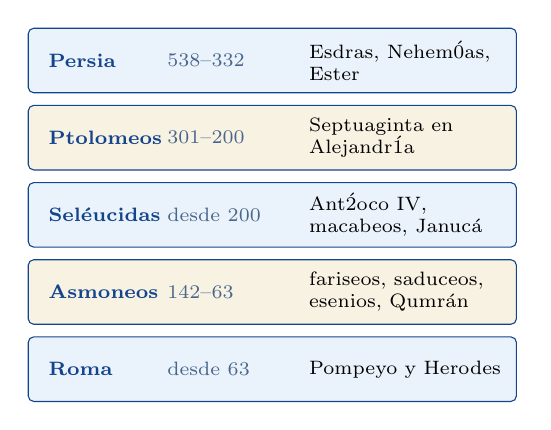
\begin{tikzpicture}[x=1cm,y=1cm]
\foreach \i/\t/\f/\d/\c in {0/{Persia}/{538--332}/{Esdras, Nehemías, Ester}/piedra,
  1/{Ptolomeos}/{301--200}/{Septuaginta en Alejandría}/oro!14!white,
  2/{Seléucidas}/{desde 200}/{Antíoco~IV, macabeos, Janucá}/piedra,
  3/{Asmoneos}/{142--63}/{fariseos, saduceos, esenios, Qumrán}/oro!14!white,
  4/{Roma}/{desde 63}/{Pompeyo y Herodes}/piedra}{
  \node[draw=ladrillo,fill=\c,rounded corners=2pt,minimum width=6.2cm,minimum height=0.82cm,anchor=north west] (r\i) at (0,{-\i*0.98}) {};
  \node[anchor=west,font=\scriptsize\bfseries,text=ladrillo] at ([xshift=4pt]r\i.west) {\t};
  \node[anchor=west,font=\scriptsize,text=sepia] at ([xshift=1.65cm]r\i.west) {\f};
  \node[anchor=west,font=\scriptsize,text width=2.6cm,align=left] at ([xshift=3.45cm]r\i.west) {\d};}
\end{tikzpicture}
\notafig{Elaboración propia. Fechas a.\,e.\,c.; cf. Dn 11.}
\end{column}
\end{columns}
\end{frame}

\begin{frame}{Alejandro y la Septuaginta}
\begin{columns}[T,onlytextwidth]
\begin{column}{0.48\textwidth}\footnotesize
\textbf{\textcolor{ladrillo}{Alejandro y sus herederos}}
\begin{itemize}
\item Iso (333), costa (332). Josefo: se postra ante el sumo sacerdote Jadúa y le muestran Daniel (\emph{Ant.} 11.329--339; cf. Yoma 69a).
\item Ptolomeos (301--200), Seléucidas desde Panias (200): «rey del sur» y «rey del norte» (Dn 11:5--20).
\end{itemize}
\begin{clave}\textbf{Precisión:} visita probablemente legendaria; ninguna fuente griega la recoge.\end{clave}
\end{column}
\begin{column}{0.48\textwidth}
\begin{notalam}[La Septuaginta: leyenda e historia]
\textbf{Leyenda.} \emph{Carta de Aristeas}: 72 sabios, 6 por tribu, en 72 días, bajo Ptolomeo~II (cf. Meguilá 9a--b).\par\smallskip
\textbf{Historia.} El Pentateuco se traduce en Alejandría en el s. \textsc{iii} a.\,e.\,c.; c. 132 el prólogo de Ben Sirá ya conoce «la ley, los profetas y los demás libros» en griego.\par\smallskip
\textbf{Memoria.} Filón: fiesta anual en Faros por la traducción (\emph{Vida de Moisés} 2.41).
\end{notalam}
\end{column}
\end{columns}
\end{frame}

\begin{frame}{Helenización y Onías III}
\begin{columns}[T,onlytextwidth]
\begin{column}{0.48\textwidth}\footnotesize
\begin{itemize}
\item \textbf{Antíoco~IV Epífanes} (175--164), hijo de Antíoco~III.\medskip
\item \textbf{Jasón} compra el sumo sacerdocio y levanta un gimnasio (2~Mac 4:7--15): «auge del helenismo» (\grc{ἀκμή τις Ἑλληνισμοῦ}).\medskip
\item Como su contrario surge la palabra \grc{Ἰουδαϊσμός}, «judaísmo» (2~Mac 2:21; 8:1; cf. Gá 1:13--14).
\end{itemize}
\end{column}
\begin{column}{0.48\textwidth}
\begin{notalam}[Onías III y Daniel]
\footnotesize\textbf{Onías~III}, sumo sacerdote legítimo, es asesinado c. 171/170 en Dafne por \textbf{Andrónico}, a instancias de \textbf{Menelao}; Antíoco ejecuta luego a Andrónico (2~Mac 4:33--38).\par\smallskip
Muchos intérpretes lo relacionan con Dn 9:26 («se quitará la vida al ungido») y 11:22 («el príncipe del pacto»).
\end{notalam}
\end{column}
\end{columns}
\end{frame}

\begin{frame}{Antíoco IV y la abominación}
\begin{columns}[T,onlytextwidth]
\begin{column}{0.46\textwidth}
\centering{\large\heb{וְנָתְנוּ הַשִּׁקּוּץ מְשׁוֹמֵם}}\par\smallskip
\begin{cita}Y quitarán el continuo sacrificio, y pondrán la abominación desoladora.\fuente{(Dn 11:31; cf. 8:9--12)}\end{cita}
\begin{notalam}[Daniel y la crisis]
Redacción tradicional s. \textsc{vi}; la crítica fecha Dn 7--12 c. 167--164 (Collins, 1993). Jesús retoma la expresión (Mt 24:15). El templo se dedica a \grc{Διὸς Ὀλυμπίου}, «Zeus Olímpico» (2~Mac 6:2).
\end{notalam}
\end{column}
\begin{column}{0.50\textwidth}
\begin{tikzpicture}[x=1cm,y=1cm]
\draw[line width=1.4pt,ladrillo] (0,0.2) -- (0,-5.3);
\foreach \i/\f/\t in {0/{169}/{Saqueo del templo (1~Mac 1:20--24)},
  1/{168}/{Roma lo frena en Eleusis (cf. Dn 11:30, «naves de Quitim»)},
  2/{167}/{Prohíbe circuncisión, sábado y Torá (1~Mac 1:41--61)},
  3/{15 kislev 167}/{\grc{βδέλυγμα ἐρημώσεως} sobre el altar (1~Mac 1:54)},
  4/{25 kislev 167}/{Primer sacrificio pagano (1~Mac 1:59)},
  5/{25 kislev 164}/{Templo purificado: Janucá (1~Mac 4:52)}}{
  \node[hito] at (0,{-\i*1.0}) {};
  \node[anchor=east,font=\scriptsize\bfseries,text=ladrillo,align=right,text width=1.3cm] at (-0.18,{-\i*1.0}) {\f};
  \node[anchor=west,font=\scriptsize,text width=4.2cm,align=left] at (0.2,{-\i*1.0}) {\t};}
\end{tikzpicture}
\notafig{Elaboración propia. Fechas a.\,e.\,c.}
\end{column}
\end{columns}
\end{frame}

\begin{frame}{Precisiones sobre la crisis}
\footnotesize\renewcommand{\arraystretch}{1.25}
\centering
\begin{tabular}{>{\RaggedRight\arraybackslash}p{3.7cm}>{\RaggedRight\arraybackslash}p{8.1cm}}
\toprule
\color{ladrillo}\bfseries Tema & \color{ladrillo}\bfseries Precisión (con fuente)\\\midrule
Filiación de Antíoco~IV & Hijo de \textbf{Antíoco~III} el Grande; hermano de Seleuco~IV\\
Orden de los dominios & Primero \textbf{Ptolomeos} (301--200), después \textbf{Seléucidas}\\
Ptolomeo~VI Filométor & Rival de su \textbf{hermano} Ptolomeo~VIII; ambos eran sobrinos de Antíoco\\
La abominación & \textbf{Zeus Olímpico} (2~Mac 6:2); 1~Mac 1:54, 59: altar pagano \emph{sobre el altar}; cerdos: Josefo, \emph{Ant.} 12.253\\
Muerte del sumo sacerdote & \textbf{Onías~III}, c. 171/170, por Andrónico y Menelao (2~Mac 4:33--35)\\
Reinauguración del templo & \textbf{25 de kislev de 164} a.\,e.\,c. (1~Mac 4:52)\\
2.300 «tardes y mañanas» & \textbf{Una lectura entre varias} (véase la lámina siguiente)\\
\bottomrule
\end{tabular}
\elabpropia
\begin{clave}Lo firme: la crisis, la rebelión de Matatías, Janucá y el hecho de que el hebreo de Dn 8:14 no diga «días».\end{clave}
\end{frame}

\begin{frame}{Las 2.300 «tardes y mañanas»}
\vspace{-4pt}\centering{\normalsize\heb{עַד עֶרֶב בֹּקֶר אַלְפַּיִם וּשְׁלֹשׁ מֵאוֹת וְנִצְדַּק קֹדֶשׁ}}\par
\begin{cita}Hasta dos mil trescientas tardes y mañanas; luego el santuario será restablecido en su derecho.\fuente{(Dn 8:14)}\end{cita}
\footnotesize\renewcommand{\arraystretch}{1.25}
\begin{tabular}{>{\RaggedRight\arraybackslash}p{2.8cm}>{\RaggedRight\arraybackslash}p{8.7cm}}
\toprule
\color{ladrillo}\bfseries Lectura & \color{ladrillo}\bfseries Cómputo\\\midrule
1.150 días & Sacrificio de la tarde y de la mañana contados por separado (unos 3 años y 2 meses)\\
2.300 días & Unos 6 años y 4 meses, desde el comienzo de la crisis (c. 171)\\
2.300 años & Interpretación historicista (día por año)\\
\bottomrule
\end{tabular}
\elabpropia
\begin{notalam}[Precisión]
1~Mac 1:54 y 4:52 dan del 15 de kislev de 167 al 25 de kislev de 164: tres años y diez días, algo menos de 1.150 días. Cf. Dn 12:11--12 (1.290 y 1.335 días).
\end{notalam}
\end{frame}

\begin{frame}{Macabeos y Janucá}
\begin{columns}[T,onlytextwidth]
\begin{column}{0.48\textwidth}
\begin{tikzpicture}[x=1cm,y=1cm]
\node[bloque,text width=5.4cm] (a) at (0,0) {\textbf{Matatías en Modín}: «todo el que tenga celo por la ley [\ldots] salga detrás de mí» (1~Mac 2:27)};
\node[bloque,text width=5.4cm] (b) at (0,-1.35) {\textbf{Judas Macabeo} vence y recupera Jerusalén};
\node[bloqueazul,text width=5.4cm] (c) at (0,-2.55) {25 de kislev de 164: altar nuevo y dedicación durante ocho días (1~Mac 4:36--59)};
\node[bloqueoro,text width=5.4cm] (d) at (0,-3.85) {Jesús en el templo en \grc{τὰ ἐγκαίνια}, «la fiesta de la dedicación» (Jn 10:22)};
\draw[flecha] (a) -- (b); \draw[flecha] (b) -- (c); \draw[flecha] (c) -- (d);
\end{tikzpicture}
\elabpropia
\end{column}
\begin{column}{0.48\textwidth}
\begin{notalam}[Ocho días: tradición y fuentes antiguas]
\footnotesize\textbf{Tradición:} una sola vasija de aceite puro, suficiente para un día, ardió ocho (Talmud, Shabat 21b).\par\medskip
\textbf{Fuentes antiguas:} 1--2~Mac no mencionan el aceite; explican los ocho días por la dedicación y por el Sucot que no se había podido celebrar (2~Mac 10:6).
\end{notalam}
\end{column}
\end{columns}
\end{frame}

\begin{frame}{De los asmoneos a Herodes}
\centering
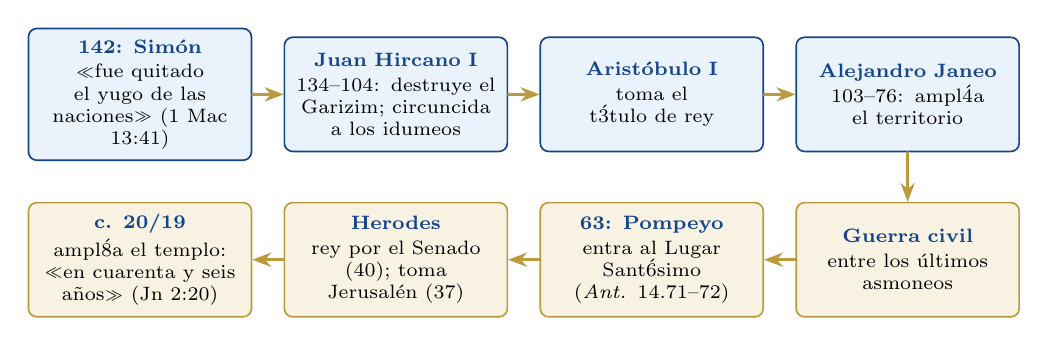
\begin{tikzpicture}[x=1cm,y=1cm]
\foreach \i/\x/\y/\t/\d/\s in {1/0/0/{142: Simón}/{«fue quitado el yugo de las naciones» (1~Mac 13:41)}/bloque,
  2/3.25/0/{Juan Hircano~I}/{134--104: destruye el Garizim; circuncida a los idumeos}/bloque,
  3/6.5/0/{Aristóbulo~I}/{toma el título de rey}/bloque,
  4/9.75/0/{Alejandro Janeo}/{103--76: amplía el territorio}/bloque,
  5/9.75/-2.1/{Guerra civil}/{entre los últimos asmoneos}/bloqueoro,
  6/6.5/-2.1/{63: Pompeyo}/{entra al Lugar Santísimo (\emph{Ant.} 14.71--72)}/bloqueoro,
  7/3.25/-2.1/{Herodes}/{rey por el Senado (40); toma Jerusalén (37)}/bloqueoro,
  8/0/-2.1/{c. 20/19}/{amplía el templo: «en cuarenta y seis años» (Jn 2:20)}/bloqueoro}{
  \node[\s,text width=2.55cm,minimum height=1.45cm] (n\i) at (\x,\y) {\textbf{\textcolor{ladrillo}{\t}}\\[1pt]\d};}
\foreach \a/\b in {1/2,2/3,3/4,5/6,6/7,7/8}{\draw[flecha] (n\a) -- (n\b);}
\draw[flecha] (n4) -- (n5);
\end{tikzpicture}
\elabpropia
\vspace{6pt}
\begin{clave}Sacerdotes no davídicos que reinan como reyes, algo que no todos aceptaron. Hag 2:9: en tamaño, Herodes superó la primera casa; la plenitud de la promesa, no.\end{clave}
\end{frame}

\begin{frame}{Fariseos, saduceos y esenios}
\centering
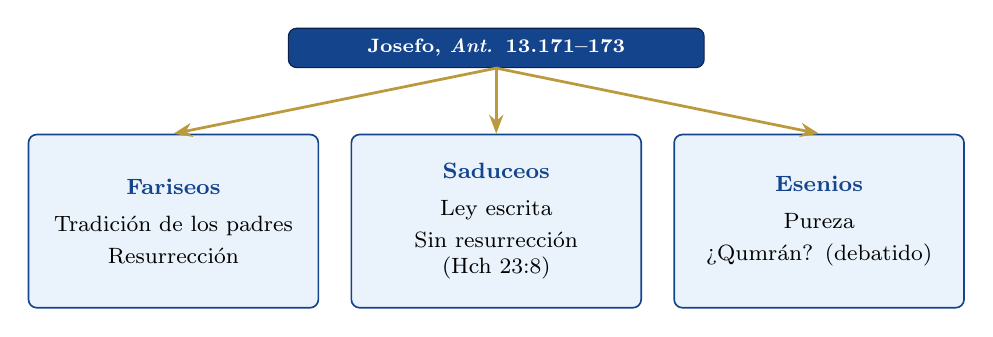
\begin{tikzpicture}[x=1cm,y=1cm]
\node[bloqueazul,text width=5.0cm] (j) at (4.1,0) {Josefo, \emph{Ant.} 13.171--173};
\foreach \i/\x/\t/\d in {1/0/{Fariseos}/{Tradición de los padres\\[2pt]Resurrección},
  2/4.1/{Saduceos}/{Ley escrita\\[2pt]Sin resurrección (Hch 23:8)},
  3/8.2/{Esenios}/{Pureza\\[2pt]¿Qumrán? (debatido)}}{
  \node[bloque,text width=3.4cm,minimum height=2.2cm,font=\footnotesize] (e\i) at (\x,-2.2) {\textbf{\textcolor{ladrillo}{\t}}\\[4pt]\d};
  \draw[flecha] (j.south) -- (e\i.north);}
\end{tikzpicture}
\elabpropia
\vspace{8pt}
\begin{notalam}[Qumrán y la espera]
\footnotesize La \emph{Regla de la comunidad} espera «la venida de un profeta y de los mesías de Aarón y de Israel» (1QS 9:11). La identificación de esta comunidad con los esenios de Josefo sigue en discusión.
\end{notalam}
\end{frame}

% ===================================================
\section{Vocación}
\begin{frame}{Pueblo santo sin rey}
\centering
\begin{tikzpicture}
 \foreach \x/\n/\t/\d/\r in {0/1/{La Torá}/{Leída, explicada y obedecida: un pueblo rehecho en torno a un libro.}/{Esd 7:10; Neh 8:1--8; Mal 2:7},
   3.15/2/{El sábado}/{Señal de identidad en todo el imperio, defendida hasta la muerte.}/{Neh 13:15--22; 1~Mac 2:29--38},
   6.3/3/{La sinagoga}/{\grc{προσευχή} en Egipto (s. \textsc{iii}); Teodoto en Jerusalén; lectura cada sábado.}/{Hch 15:21; Levine, 2005},
   9.45/4/{Las naciones}/{Prosélitos y «temerosos de Dios»: extranjeros unidos a YHWH.}/{Is 56:6--7; Hch 10:2; 13:16}}{
  \node[caja,anchor=north] (b\n) at (\x,0) {\parbox[t][3.1cm][t]{2.65cm}{\RaggedRight
    {\small\textbf{\textcolor{ladrillo}{\t}}}\\[4pt]\footnotesize \d\par\vfill{\tiny\color{sepia}(\r)}}};
  \node[circle,fill=cafe,text=piedra,font=\scriptsize\bfseries,inner sep=1.6pt] at (b\n.north west) {\n};}
\end{tikzpicture}
\elabpropia
\vspace{6pt}
\begin{clave}\small \heb{כִּי בֵיתִי בֵּית־תְּפִלָּה יִקָּרֵא לְכָל־הָעַמִּים}: «mi casa será llamada casa de oración para todos los pueblos» (Is 56:7).\end{clave}
\end{frame}

\begin{frame}{El manto de un judío}
\begin{columns}[T,onlytextwidth]
\begin{column}{0.48\textwidth}
\begin{cita}Diez hombres de todas las lenguas de las naciones se asirán del manto de un judío, diciendo: «Iremos con vosotros, porque hemos oído que Dios está con vosotros».\fuente{(Zac 8:23)}\end{cita}
\begin{notalam}[Hebreo: \heb{כָּנָף}, \emph{kanaf}]
El borde del manto con los flecos (Nm 15:38). Las naciones llegan a Dios de la mano de un israelita fiel: una tarea sacerdotal.
\end{notalam}
\end{column}
\begin{column}{0.48\textwidth}\centering
\begin{tikzpicture}[x=1cm,y=1cm]
\node[bloque,text width=4.8cm] (a) at (0,0) {\textbf{Las naciones}\\«diez hombres de todas las lenguas»};
\node[bloqueazul,text width=4.8cm] (b) at (0,-1.45) {se asen del \heb{כָּנָף} de un judío};
\node[bloqueoro,text width=4.8cm] (c) at (0,-2.9) {«Dios está con vosotros»};
\draw[flecha] (a) -- (b); \draw[flecha] (b) -- (c);
\node[bloque,text width=4.8cm,font=\scriptsize,align=left] (d) at (0,-4.35) {\textbf{Cauces:} Septuaginta (Ro 3:2), prosélitos (Mt 23:15; Hch 2:10), «temerosos de Dios» (Hch 10:2; 13:16)};
\draw[sepia,dashed] (c) -- (d);
\end{tikzpicture}
\elabpropia
\end{column}
\end{columns}
\end{frame}

\begin{frame}{El riesgo: la separación hostil}
\centering
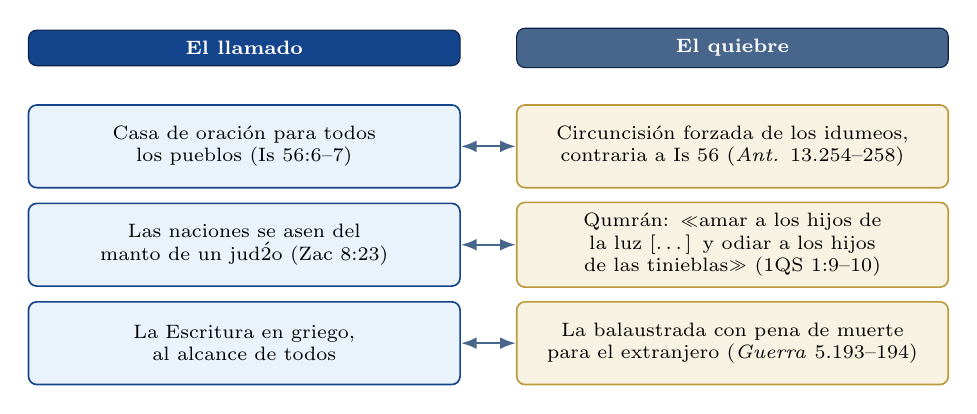
\begin{tikzpicture}[x=1cm,y=1cm]
\node[bloqueazul,text width=5.2cm] (h1) at (-3.1,0) {El llamado};
\node[bloqueazul,text width=5.2cm,fill=sepia] (h2) at (3.1,0) {El quiebre};
\foreach \i/\l/\r in {1/{Casa de oración para todos los pueblos (Is 56:6--7)}/{Circuncisión forzada de los idumeos, contraria a Is 56 (\emph{Ant.} 13.254--258)},
  2/{Las naciones se asen del manto de un judío (Zac 8:23)}/{Qumrán: «amar a los hijos de la luz [\ldots] y odiar a los hijos de las tinieblas» (1QS 1:9--10)},
  3/{La Escritura en griego, al alcance de todos}/{La balaustrada con pena de muerte para el extranjero (\emph{Guerra} 5.193--194)}}{
  \node[bloque,text width=5.2cm,minimum height=1.05cm] (l\i) at (-3.1,{-\i*1.25}) {\l};
  \node[bloqueoro,text width=5.2cm,minimum height=1.05cm] (r\i) at (3.1,{-\i*1.25}) {\r};
  \draw[sepia,line width=0.8pt,{Latex[length=2mm]}-{Latex[length=2mm]}] (l\i.east) -- (r\i.west);}
\end{tikzpicture}
\elabpropia
\vspace{6pt}
\begin{clave}Cristo «derribó el muro intermedio de separación» (\grc{τὸ μεσότοιχον τοῦ φραγμοῦ}, Ef 2:14). Israel había sido llamado a ser el lugar donde las naciones encuentran a Dios, no a cerrarles el paso.\end{clave}
\end{frame}

% ===================================================
\section{Tradición judía}
\begin{frame}{Gran Asamblea y fin de la profecía}
\centering
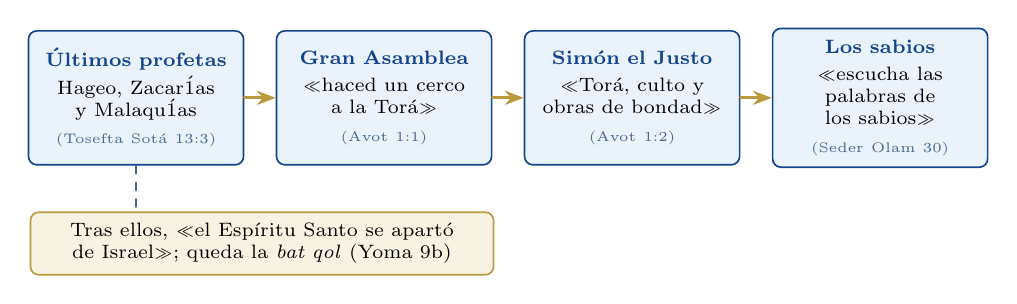
\begin{tikzpicture}[x=1cm,y=1cm]
\foreach \i/\t/\d/\r in {1/{Últimos profetas}/{Hageo, Zacarías y Malaquías}/{Tosefta Sotá 13:3},
  2/{Gran Asamblea}/{«haced un cerco a la Torá»}/{Avot 1:1},
  3/{Simón el Justo}/{«Torá, culto y obras de bondad»}/{Avot 1:2},
  4/{Los sabios}/{«escucha las palabras de los sabios»}/{Seder Olam 30}}{
  \node[bloque,text width=2.45cm,minimum height=1.7cm] (n\i) at ({(\i-1)*3.15},0) {\textbf{\textcolor{ladrillo}{\t}}\\[2pt]\d\\[2pt]{\tiny\color{sepia}(\r)}};}
\foreach \a/\b in {1/2,2/3,3/4}{\draw[flecha] (n\a.east) -- (n\b.west);}
\node[bloqueoro,text width=5.6cm,font=\scriptsize] (bq) at (1.6,-1.85) {Tras ellos, «el Espíritu Santo se apartó de Israel»; queda la \emph{bat qol} (Yoma 9b)};
\draw[sepia,dashed] (n1.south) -- (n1.south |- bq.north);
\end{tikzpicture}
\elabpropia
\begin{notalam}[Esdras en la tradición]
Lectura de la Torá lunes, jueves y sábado (Bava Kama 82a); Neh 8:8 como origen del Targum (Meguilá 3a); 120 ancianos ordenan la Amidá (Meguilá 17b). Son lecturas tradicionales: la Gran Asamblea como institución histórica está en discusión.
\end{notalam}
\end{frame}

\begin{frame}{Amidá: la reunión de los dispersos}
\centering{\heb{תְּקַע בְּשׁוֹפָר גָּדוֹל לְחֵרוּתֵנוּ וְשָׂא נֵס לְקַבֵּץ גָּלֻיּוֹתֵינוּ}}\par\smallskip
\begin{cita}Toca el gran shofar por nuestra libertad, alza estandarte para reunir a nuestros desterrados [\ldots]. Bendito eres tú, YHWH, que reúnes a los dispersos de tu pueblo Israel.\fuente{(Amidá, décima bendición)}\end{cita}
\vspace{4pt}
\begin{notalam}[Precisión]
\footnotesize El texto actual de la Amidá es posterior a 70 e.\,c., pero su esperanza ya estaba viva en el Segundo Templo. En Is 11:12, «Israel» es el reino del norte y «Judá» el del sur; la Amidá dice «tu pueblo Israel», el pueblo entero.
\end{notalam}
\end{frame}

\begin{frame}{De Isaías a la Amidá}
\centering
\begin{tikzpicture}[x=0.96cm,y=1cm]
\node[bloque,text width=3.5cm] (a) at (0,1.3) {\textbf{Is 27:13}\\«se tocará el gran shofar»};
\node[bloque,text width=3.5cm] (b) at (0,0) {\textbf{Is 11:12}\\desterrados de \textbf{Israel} (norte) y esparcidos de \textbf{Judá} (sur)};
\node[bloque,text width=3.5cm] (c) at (0,-1.3) {\textbf{Is 56:8}\\\heb{מְקַבֵּץ נִדְחֵי יִשְׂרָאֵל}};
\node[bloqueazul,text width=2.4cm,minimum height=1.6cm] (m) at (4.6,0) {Amidá,\\décima bendición};
\node[bloqueoro,text width=3.4cm] (d) at (9.0,0.75) {\textbf{Eclo 36:10} (c. 180)\\«reúne a todas las tribus de Jacob»};
\node[bloqueoro,text width=3.4cm] (e) at (9.0,-0.85) {\textbf{Eclo 48:10}\\Elías, \grc{καταστῆσαι φυλὰς Ἰακώβ}};
\draw[flecha] (a.east) -- (m.west); \draw[flecha] (b.east) -- (m.west); \draw[flecha] (c.east) -- (m.west);
\draw[sepia,dashed] (m.east) -- (d.west); \draw[sepia,dashed] (m.east) -- (e.west);
\node[etiq,font=\scriptsize\itshape,text=sepia] at (0,2.15) {Fuentes proféticas};
\node[etiq,font=\scriptsize\itshape,text=sepia] at (9.0,2.15) {La misma esperanza, antes de 70};
\end{tikzpicture}
\elabpropia
\vspace{6pt}
\begin{clave}Para Ben Sirá, el retorno de Babilonia no había sido la reunión plena de las tribus: une Mal 4:6 [3:24] con Is 49:6.\end{clave}
\end{frame}

\begin{frame}{Purim, Janucá, Seder Olam y Josefo}
\begin{columns}[T,onlytextwidth]
\begin{column}{0.48\textwidth}
\textbf{\small\textcolor{ladrillo}{Dos fiestas nuevas}}\par\smallskip
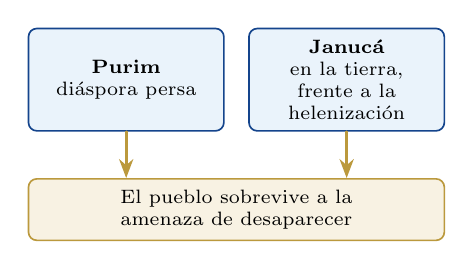
\begin{tikzpicture}[x=1cm,y=1cm]
\node[bloque,text width=2.2cm,minimum height=1.3cm] (p) at (0,0) {\textbf{Purim}\\diáspora persa};
\node[bloque,text width=2.2cm,minimum height=1.3cm] (j) at (2.8,0) {\textbf{Janucá}\\en la tierra, frente a la helenización};
\node[bloqueoro,text width=5.0cm] (s) at (1.4,-1.65) {El pueblo sobrevive a la amenaza de desaparecer};
\draw[flecha] (p) -- (p |- s.north); \draw[flecha] (j) -- (j |- s.north);
\end{tikzpicture}
\elabpropia
\vspace{4pt}
{\footnotesize \emph{Al ha-nisim}: «el reino malvado de Grecia se levantó contra tu pueblo Israel para hacerles olvidar tu Torá».}
\end{column}
\begin{column}{0.48\textwidth}
\textbf{\small\textcolor{ladrillo}{Cronología corta}}\par\smallskip
\footnotesize\renewcommand{\arraystretch}{1.25}
\begin{tabular}{>{\RaggedRight\arraybackslash}p{1.75cm}>{\RaggedRight\arraybackslash}p{1.3cm}>{\RaggedRight\arraybackslash}p{1.95cm}}
\toprule
\color{ladrillo}\bfseries Período & \color{ladrillo}\bfseries Talmud & \color{ladrillo}\bfseries Historia\\\midrule
Persia & 34 años & c. 200 años\\
Grecia & 180 & \\
Asmoneos & 103 & \\
Herodes & 103 & \\
\midrule
Total & 420 & 515 a.\,e.\,c.--70 e.\,c.\\
\bottomrule
\end{tabular}
\notafig{Elaboración propia a partir de Avodá Zará 9a y Seder Olam 30 (Guggenheimer, 1998). Fuente histórica principal: Josefo, \emph{Antigüedades} 11--17.}
\end{column}
\end{columns}
\end{frame}

% ===================================================
\section{Restauración}
\begin{frame}{Un retorno real pero parcial}
\begin{columns}[T,onlytextwidth]
\begin{column}{0.44\textwidth}
\centering{\heb{הִנֵּה אֲנַחְנוּ הַיּוֹם עֲבָדִים}}\par\smallskip
\begin{cita}He aquí que hoy somos siervos [\ldots] y su abundante fruto es para los reyes que has puesto sobre nosotros.\fuente{(Neh 9:36--37)}\end{cita}
\begin{clave}Tob 14:5: reconstruirán el templo, «pero no como el primero, hasta que se cumplan los tiempos».\end{clave}
\end{column}
\begin{column}{0.52\textwidth}\centering
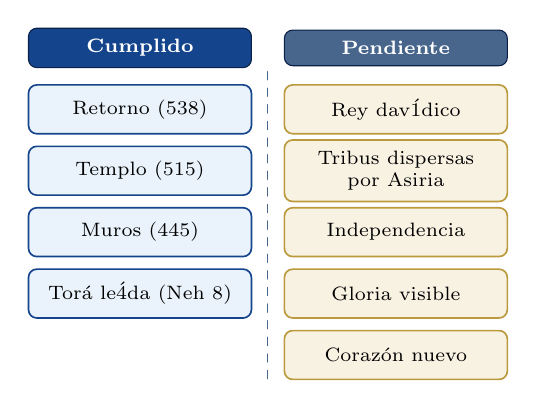
\begin{tikzpicture}[x=1cm,y=1cm]
\node[bloqueazul,text width=2.55cm] (h1) at (0,0) {Cumplido};
\node[bloqueazul,text width=2.55cm,fill=sepia] (h2) at (3.25,0) {Pendiente};
\foreach \i/\t in {1/{Retorno (538)},2/{Templo (515)},3/{Muros (445)},4/{Torá leída (Neh 8)}}{
  \node[bloque,text width=2.55cm,minimum height=0.62cm] at (0,{-\i*0.78}) {\t};}
\foreach \i/\t in {1/{Rey davídico},2/{Tribus dispersas por Asiria},3/{Independencia},4/{Gloria visible},5/{Corazón nuevo}}{
  \node[bloqueoro,text width=2.55cm,minimum height=0.62cm] at (3.25,{-\i*0.78}) {\t};}
\draw[sepia,dashed] (1.625,-0.3) -- (1.625,-4.3);
\end{tikzpicture}
\elabpropia
\end{column}
\end{columns}
\end{frame}

\begin{frame}{Setenta años, setenta semanas}
\begin{columns}[T,onlytextwidth]
\begin{column}{0.46\textwidth}
\centering{\heb{שָׁבֻעִים שִׁבְעִים נֶחְתַּךְ עַל־עַמְּךָ}}\par\smallskip
\begin{cita}[fontupper=\footnotesize\itshape]Setenta semanas están determinadas sobre tu pueblo y sobre tu santa ciudad, para terminar la prevaricación [\ldots] y traer la justicia perdurable.\fuente{(Dn 9:24)}\end{cita}
\begin{notalam}[Debate: ¿un «exilio continuado»?]
N.~T. Wright (1992) sostiene que muchos judíos del Segundo Templo se veían aún en el exilio. Su alcance se discute, pero Neh 9, Dn 9 y Tob 14 la respaldan en lo esencial.
\end{notalam}
\end{column}
\begin{column}{0.50\textwidth}\centering
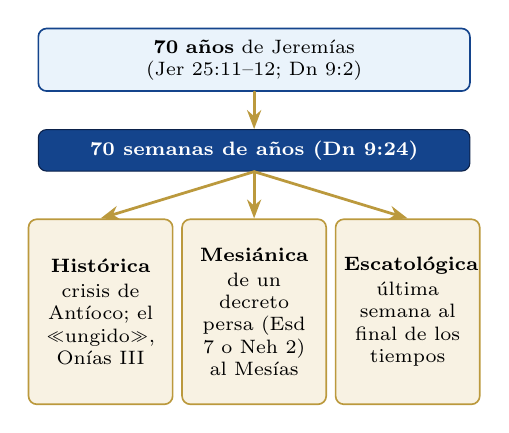
\begin{tikzpicture}[x=1cm,y=1cm]
\node[bloque,text width=5.2cm] (a) at (0,0) {\textbf{70 años} de Jeremías (Jer 25:11--12; Dn 9:2)};
\node[bloqueazul,text width=5.2cm] (b) at (0,-1.15) {\textbf{70 semanas} de años (Dn 9:24)};
\node[bloqueoro,text width=1.62cm,minimum height=2.35cm,font=\scriptsize,inner sep=3pt] (c1) at (-1.95,-3.2) {\textbf{Histórica}\\[1pt]crisis de Antíoco; el «ungido», Onías~III};
\node[bloqueoro,text width=1.62cm,minimum height=2.35cm,font=\scriptsize,inner sep=3pt] (c2) at (0,-3.2) {\textbf{Mesiánica}\\[1pt]de un decreto persa (Esd 7 o Neh 2) al Mesías};
\node[bloqueoro,text width=1.62cm,minimum height=2.35cm,font=\scriptsize,inner sep=3pt] (c3) at (1.95,-3.2) {\textbf{Escatológica}\\[1pt]última semana al final de los tiempos};
\draw[flecha] (a) -- (b);
\foreach \k in {1,2,3}{\draw[flecha] (b.south) -- (c\k.north);}
\end{tikzpicture}
\notafig{Elaboración propia a partir de Collins (1993).}
\end{column}
\end{columns}
\end{frame}

\begin{frame}{Isaías: más de lo que se vio en 538}
\centering\footnotesize\renewcommand{\arraystretch}{1.2}
\begin{tabular}{>{\RaggedRight\arraybackslash}p{1.8cm}>{\RaggedRight\arraybackslash}p{5.6cm}>{\RaggedRight\arraybackslash}p{4.0cm}}
\toprule
\color{ladrillo}\bfseries Texto & \color{ladrillo}\bfseries Promesa & \color{ladrillo}\bfseries Recepción\\\midrule
Is 2:2--4 & Las naciones suben al monte de YHWH & Zac 8:20--22\\
Is 11:11--12 & Israel (norte) y Judá (sur) reunidos «por segunda vez» & Amidá 10; Eclo 36:10\\
Is 44:28--45:1 & Ciro reconstruye & Esd 1: cumplido\\
Is 49:5--6 & Levantar las tribus de Jacob y luz de las naciones & Eclo 48:10; Lc 2:32; Hch 13:47\\
Is 56:6--8 & Extranjeros en el templo; «aún juntaré a otros» & Mc 11:17\\
Is 60--62 & Naciones a la luz de Sion; «sacerdotes de YHWH» & Ro 11:12, 15\\
Is 66:18--23 & Mensajeros a las naciones; sacerdotes de ellas & Ro 15:16\\
\bottomrule
\end{tabular}
\elabpropia
\end{frame}

\begin{frame}{Is 49:6: las tribus y las naciones}
\begin{columns}[T,onlytextwidth]
\begin{column}{0.46\textwidth}
\begin{cita}Poco es que seas mi siervo para levantar las tribus de Jacob [\ldots]; también te di por luz de las naciones (\upshape\heb{לְאוֹר גּוֹיִם}\itshape).\fuente{(Is 49:6)}\end{cita}
\begin{clave}Levantar a las tribus y alumbrar a las naciones forman una sola obra. Simeón citará el texto ante el niño Jesús (Lc 2:32).\end{clave}
\end{column}
\begin{column}{0.50\textwidth}\centering
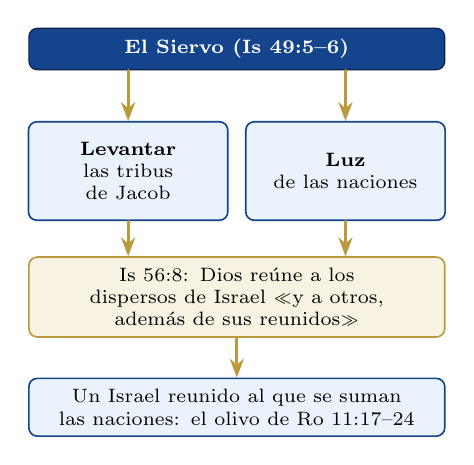
\begin{tikzpicture}[x=1cm,y=1cm]
\node[bloqueazul,text width=5.0cm] (s) at (0,0) {El Siervo (Is 49:5--6)};
\node[bloque,text width=2.25cm,minimum height=1.25cm] (t) at (-1.38,-1.55) {\textbf{Levantar}\\las tribus de Jacob};
\node[bloque,text width=2.25cm,minimum height=1.25cm] (n) at (1.38,-1.55) {\textbf{Luz}\\de las naciones};
\node[bloqueoro,text width=5.0cm] (r) at (0,-3.15) {Is 56:8: Dios reúne a los dispersos de Israel «y a otros, además de sus reunidos»};
\node[bloque,text width=5.0cm] (o) at (0,-4.55) {Un Israel reunido al que se suman las naciones: el olivo de Ro 11:17--24};
\draw[flecha] (s.south -| t.north) -- (t.north);
\draw[flecha] (s.south -| n.north) -- (n.north);
\draw[flecha] (t.south) -- (t.south |- r.north);
\draw[flecha] (n.south) -- (n.south |- r.north);
\draw[flecha] (r) -- (o);
\end{tikzpicture}
\elabpropia
\end{column}
\end{columns}
\end{frame}

\begin{frame}{Jeremías: setenta años y algo más}
\begin{columns}[T,onlytextwidth]
\begin{column}{0.48\textwidth}
\begin{cita}Cuando se cumplan en Babilonia los setenta años, yo os visitaré [\ldots]. Me buscaréis y me hallaréis, porque me buscaréis de todo vuestro corazón [\ldots] y os reuniré de todas las naciones.\fuente{(Jer 29:10, 13--14)}\end{cita}
\begin{clave}Con Ciro se cumplen los «setenta años»; «de todo corazón» y «de todas las naciones» siguen abiertos (Dn 9).\end{clave}
\end{column}
\begin{column}{0.48\textwidth}\footnotesize
\begin{itemize}
\item \textbf{Jer 33:14--17}: la buena palabra a «la casa de Israel y la casa de Judá»; el Renuevo de David; \heb{לֹא־יִכָּרֵת לְדָוִד אִישׁ}, «no faltará a David varón» en el trono.\medskip
\item En el Segundo Templo no reina ningún davídico: Zorobabel gobernador, asmoneos levitas, Herodes idumeo.\medskip
\item \textbf{Jer 3:18; 50:4--5}: Judá e Israel vendrán juntos del norte, algo que tampoco ocurrió con Ciro.
\end{itemize}
\end{column}
\end{columns}
\end{frame}

\begin{frame}{La esperanza mesiánica}
\centering
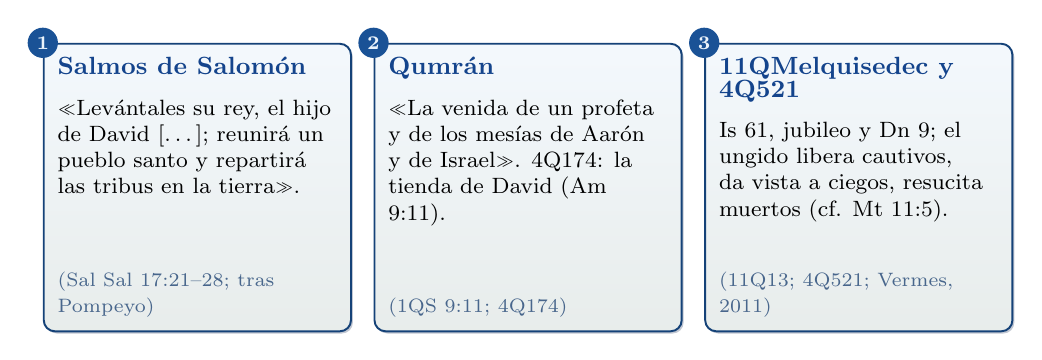
\begin{tikzpicture}
 \foreach \x/\n/\t/\d/\r in {0/1/{Salmos de Salomón}/{«Levántales su rey, el hijo de David [\ldots]; reunirá un pueblo santo y repartirá las tribus en la tierra».}/{Sal Sal 17:21--28; tras Pompeyo},
   4.2/2/{Qumrán}/{«La venida de un profeta y de los mesías de Aarón y de Israel». 4Q174: la tienda de David (Am 9:11).}/{1QS 9:11; 4Q174},
   8.4/3/{11QMelquisedec y 4Q521}/{Is 61, jubileo y Dn 9; el ungido libera cautivos, da vista a ciegos, resucita muertos (cf. Mt 11:5).}/{11Q13; 4Q521; Vermes, 2011}}{
  \node[caja,anchor=north] (b\n) at (\x,0) {\parbox[t][3.3cm][t]{3.55cm}{\RaggedRight
    {\small\textbf{\textcolor{ladrillo}{\t}}}\\[5pt]\footnotesize \d\par\vfill{\scriptsize\color{sepia}(\r)}}};
  \node[circle,fill=cafe,text=piedra,font=\scriptsize\bfseries,inner sep=1.6pt] at (b\n.north west) {\n};}
\end{tikzpicture}
\elabpropia
\vspace{8pt}
\begin{clave}\small Al final del período, Hijo de David, pueblo santo y doce tribus forman una sola esperanza.\end{clave}
\end{frame}

\begin{frame}{Simeón y Ana}
\fotolado{panel_lc2.jpg}{Elaboración propia: Lc 2:25 en escritura uncial (texto NA28).}
\begin{columns}[c,onlytextwidth]
\begin{column}{0.57\textwidth}
\begin{cita}Este hombre, justo y piadoso, esperaba la consolación de Israel, y el Espíritu Santo estaba sobre él.\fuente{(Lc 2:25)}\end{cita}
\scriptsize
\begin{itemize}
\item \grc{παράκλησιν τοῦ Ἰσραήλ}: eco de Is 40:1 (LXX \grc{παρακαλεῖτε}).
\item Ana, de la tribu de \textbf{Aser}: «la redención de Jerusalén» (Lc 2:38).
\item Hch 1:6: \grc{ἀποκαθιστάνεις τὴν βασιλείαν τῷ Ἰσραήλ;}
\item Hch 26:7: «nuestras doce tribus» (\grc{τὸ δωδεκάφυλον ἡμῶν}) esperan la promesa.
\item Gá 4:4: \grc{τὸ πλήρωμα τοῦ χρόνου}; cf. \grc{πλήρωμα} en Ro 11:12, 25.
\end{itemize}
\end{column}
\begin{column}{0.41\textwidth}\end{column}
\end{columns}
\end{frame}

% ===================================================
\section{Síntesis}
\begin{frame}{Síntesis}
\begin{tcolorbox}[colback=piedra,colframe=ladrillo,boxrule=1pt,arc=3pt,fontupper=\small]
\textbf{\textcolor{cafe}{Israel en el Segundo Templo:}} un remanente, sobre todo de Judá y Benjamín, vuelve y ofrece por las doce tribus. Sin rey, aprende a ser pueblo santo en torno a la Torá, el sábado y la sinagoga, y pone la Escritura en griego al alcance de las naciones. El retorno es verdadero pero parcial: la reunión, el rey davídico y la gloria quedan pendientes hasta «el cumplimiento del tiempo» (Gá 4:4).
\end{tcolorbox}
\centering\footnotesize\renewcommand{\arraystretch}{1.25}
\begin{tabular}{>{\RaggedRight\arraybackslash}p{2.4cm}>{\RaggedRight\arraybackslash}p{9.3cm}}
\toprule
\color{ladrillo}\bfseries Eje & \color{ladrillo}\bfseries Lo que deja esta etapa\\\midrule
Retorno real & Esd 1:1--4; 6:17; Hag 2:9; Neh 8\\
Retorno parcial & Neh 9:36--37; Dn 9:24; Tob 14:5; Zac 8:13 (dos casas aún por reunir)\\
Vocación & Torá, sábado, sinagoga, LXX, prosélitos; riesgo de separación hostil\\
Proyección & Is 49:6; Jer 33:14--17; Mal 3:1; 4:5--6; Lc 2:25; Hch 26:7; Ro 11:26--27\\
\bottomrule
\end{tabular}
\elabpropia
\end{frame}

\begin{frame}{Hacia el Estudio 7}
\begin{columns}[c,onlytextwidth]
\begin{column}{0.52\textwidth}
\begin{cita}Irá delante de él con el espíritu y el poder de Elías, para hacer volver los corazones de los padres a los hijos.\fuente{(Lc 1:17; cf. Mal 4:6 [3:24])}\end{cita}
\small En el templo de Herodes, el anuncio a Zacarías retoma a Malaquías: \destacar{se rompe el silencio}.
\end{column}
\begin{column}{0.44\textwidth}
\begin{tcolorbox}[colback=cafe,colframe=cafeosc,coltext=piedra,boxrule=0.8pt,arc=3pt,fontupper=\small]
\textbf{Estudio 7}\par\smallskip
De Cristo a la destrucción del templo: el Mesías en su contexto judío, el remanente creyente, la iglesia de Jerusalén y la caída del templo (70 e.\,c.).
\end{tcolorbox}
\end{column}
\end{columns}
\end{frame}

\begin{frame}{Para la reflexión}
\small
\begin{enumerate}
\item Un remanente de Judá y Benjamín ofreció doce machos cabríos «por todo Israel» (Esd 6:17). ¿Qué enseña sobre la relación entre el remanente y el pueblo entero (Ro 11:5, 16)?\medskip
\item Nehemías ora «hoy somos siervos» en plena restauración. ¿En qué se distingue un cumplimiento real de uno pleno?\medskip
\item ¿Qué actitudes favorecían la escena de Zac 8:23 y cuáles la impedían? ¿Qué dice esto a los creyentes de las naciones (Ro 11:18)?\medskip
\item ¿Qué cambia en Hch 1:6 al recordar que la Amidá pide cada día la reunión de los dispersos de Israel?
\end{enumerate}
\end{frame}

% ===================================================
\section{Glosario}
\begin{frame}{Glosario}
\begin{columns}[t,onlytextwidth]
\begin{column}{0.49\textwidth}\scriptsize
\textbf{Amaná} (\heb{אֲמָנָה}): pacto escrito (Neh 9:38 [10:1]).\par\smallskip
\textbf{Anshei Knéset ha-Guedolá}: hombres de la Gran Asamblea (Avot 1:1).\par\smallskip
\textbf{Bat qol} (\heb{בַּת קוֹל}): «hija de la voz»; voz del cielo tras la profecía.\par\smallskip
\textbf{Diáspora} (\grc{διασπορά}): dispersión fuera de la tierra (Stg 1:1).\par\smallskip
\textbf{Enkainia / Janucá} (\grc{τὰ ἐγκαίνια}; \heb{חֲנֻכָּה}): dedicación (Jn 10:22).\par\smallskip
\textbf{Mashíaj} (\heb{מָשִׁיחַ}): ungido; Ciro en Is 45:1.
\end{column}
\begin{column}{0.49\textwidth}\scriptsize
\textbf{Mityahadim} (\heb{מִתְיַהֲדִים}): «se hacían judíos» (Est 8:17).\par\smallskip
\textbf{Pleroma} (\grc{πλήρωμα}): plenitud (Gá 4:4; Ro 11:12, 25).\par\smallskip
\textbf{Prosélito} (\grc{προσήλυτος}): extranjero incorporado; hebreo \heb{גֵּר}.\par\smallskip
\textbf{Shiqquts meshomem} (\heb{שִׁקּוּץ מְשׁוֹמֵם}): abominación desoladora (Dn 11:31).\par\smallskip
\textbf{Sofer} (\heb{סוֹפֵר}): escriba; Esdras (Esd 7:6).\par\smallskip
\textbf{Yehud / yehudí} (\heb{יְהוּד}, \heb{יְהוּדִי}): provincia persa; «judío».
\end{column}
\end{columns}
\end{frame}

% ===================================================
\section{Referencias}
\begin{frame}[allowframebreaks]{Referencias}
\tiny
\refapa{Bickerman, E.~J. (1988). \emph{The Jews in the Greek age}. Harvard University Press.}
\refapa{\emph{Biblia Hebraica Stuttgartensia} (5.ª ed.). (1997). Deutsche Bibelgesellschaft.}
\refapa{Charlesworth, J.~H. (Ed.). (1985). \emph{The Old Testament pseudepigrapha} (Vol. 2). Doubleday.}
\refapa{Collins, J.~J. (1993). \emph{Daniel} (Hermeneia). Fortress Press.}
\refapa{Cotton, H.~M., \& Wörrle, M. (2007). Seleukos IV to Heliodoros: A new dossier of royal correspondence from Israel. \emph{Zeitschrift für Papyrologie und Epigraphik, 159}, 191--205.}
\refapa{Crown, A.~D. (Ed.). (1989). \emph{The Samaritans}. Mohr Siebeck.}
\refapa{Danby, H. (Trad.). (1933). \emph{The Mishnah}. Oxford University Press.}
\refapa{Epstein, I. (Ed.). (1935--1948). \emph{The Babylonian Talmud}. Soncino Press.}
\refapa{Finkel, I. (Ed.). (2013). \emph{The Cyrus Cylinder: The king of Persia's proclamation from ancient Babylon}. I.\,B. Tauris.}
\refapa{Finkelstein, I. (2008). Jerusalem in the Persian (and early Hellenistic) period and the wall of Nehemiah. \emph{Journal for the Study of the Old Testament, 32}(4), 501--520.}
\refapa{Goldstein, J.~A. (1976). \emph{I Maccabees} (Anchor Bible 41). Doubleday.}
\refapa{Guggenheimer, H.~W. (1998). \emph{Seder Olam: The rabbinic view of biblical chronology}. Jason Aronson.}
\refapa{Jobes, K.~H., \& Silva, M. (2015). \emph{Invitation to the Septuagint} (2.ª ed.). Baker Academic.}
\refapa{Josefo, F. (1987). \emph{The works of Josephus} (W. Whiston, Trad.). Hendrickson.}
\refapa{Kloppenborg, J.~S. (2000). Dating Theodotos (CIJ II 1404). \emph{Journal of Jewish Studies, 51}(2), 243--280.}
\refapa{Kuhrt, A. (1983). The Cyrus Cylinder and Achaemenid imperial policy. \emph{Journal for the Study of the Old Testament, 8}(25), 83--97.}
\refapa{Levine, L.~I. (2005). \emph{The ancient synagogue: The first thousand years} (2.ª ed.). Yale University Press.}
\refapa{Lipschits, O., \& Vanderhooft, D.~S. (2011). \emph{The Yehud stamp impressions}. Eisenbrauns.}
\refapa{Magen, Y. (2008). \emph{Mount Gerizim excavations: Vol. 2. A temple city}. Israel Antiquities Authority.}
\refapa{Mazar, B. (1975). \emph{The mountain of the Lord}. Doubleday.}
\refapa{Meshorer, Y. (2001). \emph{A treasury of Jewish coins: From the Persian period to Bar Kokhba}. Amphora Books; Yad Ben-Zvi Press.}
\refapa{Neusner, J. (Trad.). (2002). \emph{The Tosefta}. Hendrickson.}
\refapa{\emph{Novum Testamentum Graece} (28.ª ed.). (2012). Deutsche Bibelgesellschaft.}
\refapa{ONE FOR ISRAEL Ministry. (2025, 3 de julio). \emph{What does «all Israel will be saved» mean in Romans 11?} \url{https://www.oneforisrael.org/what-does-all-israel-will-be-saved-mean-in-romans-11/}}
\refapa{Pearce, L.~E., \& Wunsch, C. (2014). \emph{Documents of Judean exiles and West Semitic exiles in Babylonia in the collection of David Sofer} (CUSAS 28). CDL Press.}
\refapa{Porten, B., \& Yardeni, A. (1986). \emph{Textbook of Aramaic documents from ancient Egypt: Vol. 1. Letters}. Hebrew University.}
\refapa{Rahlfs, A., \& Hanhart, R. (Eds.). (2006). \emph{Septuaginta} (ed. rev.). Deutsche Bibelgesellschaft.}
\refapa{Sacks, J. (Trad.). (2009). \emph{The Koren Siddur}. Koren Publishers.}
\refapa{Schürer, E. (1973--1987). \emph{The history of the Jewish people in the age of Jesus Christ} (G. Vermes, F. Millar y M. Goodman, Eds. rev.; 3 vols.). T\&T Clark.}
\refapa{Ulrich, E., \& Flint, P.~W. (2010). \emph{Qumran Cave 1.II: The Isaiah scrolls} (DJD 32). Clarendon Press.}
\refapa{VanderKam, J.~C. (2010). \emph{The Dead Sea scrolls today} (2.ª ed.). Eerdmans.}
\refapa{Vermes, G. (2011). \emph{The complete Dead Sea scrolls in English} (ed. rev.). Penguin.}
\refapa{Williamson, H.~G.~M. (1985). \emph{Ezra, Nehemiah} (Word Biblical Commentary 16). Word Books.}
\refapa{Wright, N.~T. (1992). \emph{The New Testament and the people of God}. Fortress Press.}
\refapa{Wright, R.~B. (1985). Psalms of Solomon. En J.~H. Charlesworth (Ed.), \emph{The Old Testament pseudepigrapha} (Vol. 2). Doubleday.}
\end{frame}
\end{document}
